Engine phải trả lời ba câu hỏi với mỗi ảnh hoặc video: đối tượng cần che nằm ở đâu, đối tượng nào thuộc danh sách miễn che, và quyết định đó có giữ được qua các khung hình hay không. Chương này trình bày dữ liệu, cách đánh giá và kết quả cho từng câu hỏi, lần lượt từ phát hiện, đọc biển số, xác minh khuôn mặt đến video.

\subsection{Dữ liệu huấn luyện và đánh giá}

Trong bốn bài toán, nhóm chỉ tự huấn luyện bộ phát hiện khuôn mặt và biển số. Bộ trích đặc trưng khuôn mặt, YuNet và PP-OCRv4 dùng trọng số có sẵn, nên dữ liệu của hai bài toán này chỉ để chọn cách dùng và đánh giá. Bảng~\ref{tab:4-1} liệt kê các tập dữ liệu.

{\bangfont
\begin{longtable}{|L{2.0cm}|L{3.8cm}|L{3.6cm}|L{5.2cm}|}
\caption{Thống kê các tập dữ liệu sử dụng}\label{tab:4-1}\\
\hline
\dongdau \textbf{Bài toán} & \textbf{Tập dữ liệu} & \textbf{Quy mô} & \textbf{Vai trò} \\ \hline
\endfirsthead
\multicolumn{4}{c}{\textbf{Bảng 4.1.} (tiếp theo)}\\[2pt]
\hline
\dongdau \textbf{Bài toán} & \textbf{Tập dữ liệu} & \textbf{Quy mô} & \textbf{Vai trò} \\ \hline
\endhead
\endfoot
\endlastfoot
Phát hiện & WIDER FACE train & 12.225 ảnh & Huấn luyện lớp mặt \\ \cline{2-4}
 & Ô cắt từ ảnh đám đông & 236 ô từ 45 ảnh & Huấn luyện, từ bước 3 \\ \cline{2-4}
 & Biển số Việt Nam & 3.428 ảnh & Huấn luyện lớp biển \\ \cline{2-4}
 & Khung camera hành trình & 468 khung, 590 biển & Huấn luyện, bước 8 \\ \cline{2-4}
 & Ảnh đồng hồ xe, không nhãn & 384 ảnh & Mẫu âm của một biến thể bước 8 (bị loại) \\ \cline{2-4}
 & Validation & 610 ảnh mặt, 1.141 ảnh biển & Theo dõi trong lúc huấn luyện \\ \cline{2-4}
 & Bộ đánh giá & 3.226 ảnh WIDER val (39.112 mặt), 500 ảnh biển UET & So sánh mô hình, chọn ngưỡng \\ \hline
Đọc biển số & Tập UET & 80 biển (16 biển hai dòng) & Chọn và kiểm tra cách đọc \\ \cline{2-4}
 & Tập trungdinh & 536 biển (440 biển hai dòng) & So sánh các cách đọc \\ \hline
Xác minh mặt & LFW & 600 chủ thể, 600 người lạ, 3.000 ảnh & Chọn cách căn chỉnh và ngưỡng \\ \hline
Video & 2 clip dashcam, 3 clip điện thoại & 5.952 khung & Tìm lỗi của Engine, đánh giá toàn luồng \\ \hline
\end{longtable}
}

\textbf{Dữ liệu phát hiện.} WIDER FACE (Yang và cộng sự, 2016) có rất nhiều mặt nhỏ và mặt bị che khuất, nhóm tách 5\% phần train làm validation. Có 45 ảnh đám đông trên 300 mặt làm tràn bộ nhớ GPU ở 1280 px, nên nhóm bỏ ở các bước đầu rồi đưa lại dưới dạng 236 ô cắt. Với biển số, chín ảnh gần trùng với bộ đánh giá đã được loại. Bộ đánh giá 3.726 ảnh không tham gia cập nhật trọng số, nhưng nhóm dùng chính nó để so mô hình và chọn ngưỡng. Vì vậy các con số có thể hơi lạc quan so với một tập hoàn toàn mới, và đây là hạn chế của đề tài.

Khung dashcam được thêm vào vì kích thước biển trong dữ liệu cũ khác xa thực tế. Biển trong tập huấn luyện là ảnh cận cảnh, rộng trung bình khoảng 21\% chiều rộng ảnh (trong bộ đánh giá là 18\%), còn trên dashcam chỉ 3,2\%, và 76\% số biển nhỏ hơn 5\%. Trong 468 khung, 250 khung lấy từ BDD100K (120 khung ban đêm) và 218 khung từ hai clip giao thông Việt Nam. Nhãn do mô hình sinh trước rồi được sửa tay trên CVAT. Hai clip này không dùng trong đánh giá video.

\begin{figure}[!htp]
\centering
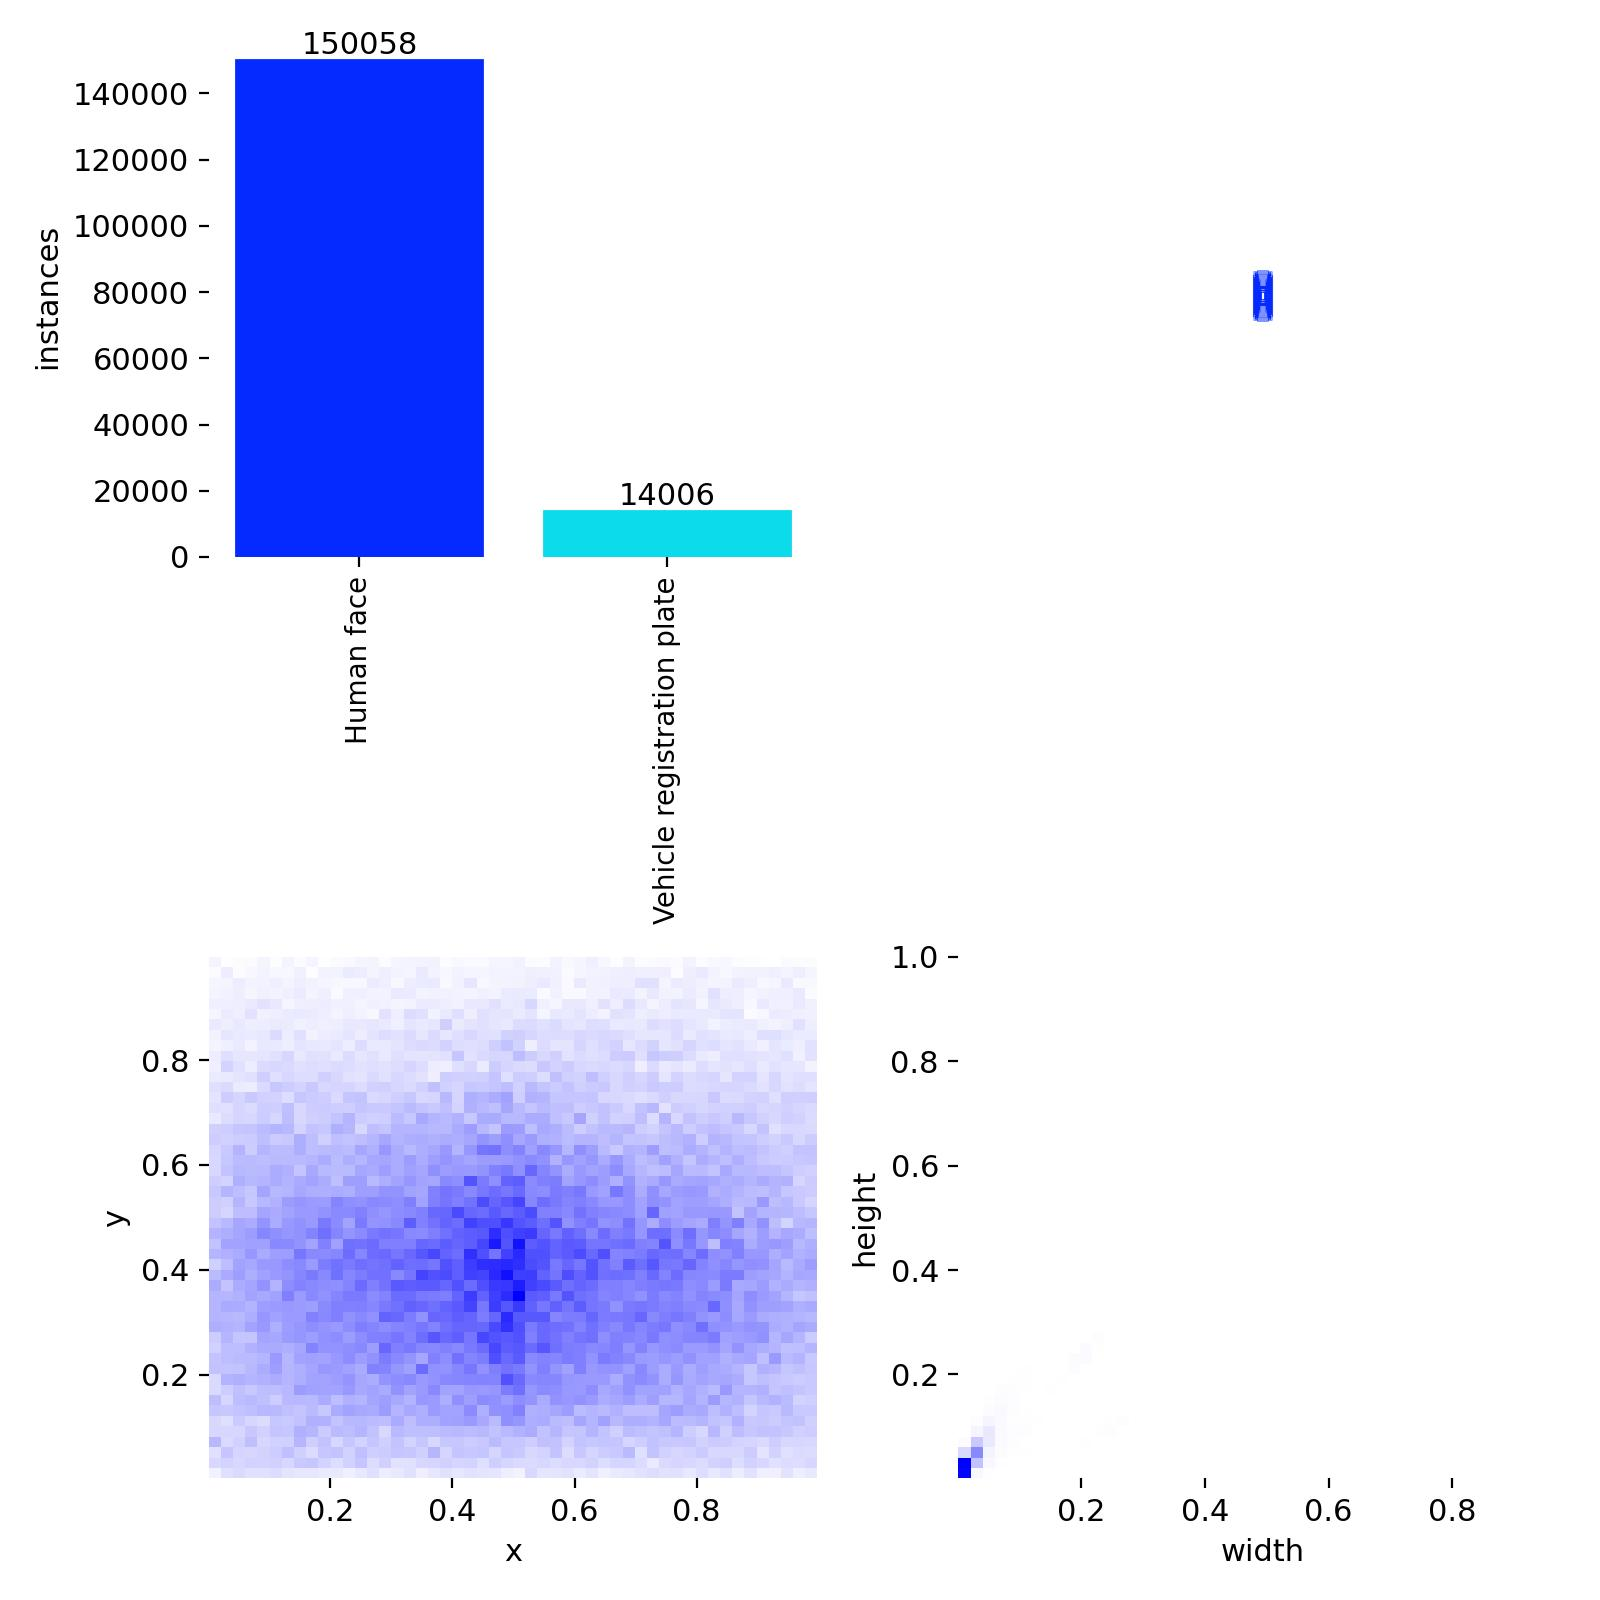
\includegraphics[width=0.72\textwidth]{figures/hinh-4-1-phan-bo-nhan.jpg}
\caption[Phân bố nhãn của tập huấn luyện]{Phân bố nhãn khi huấn luyện YOLO26s e5-dashcam: 150.058 hộp mặt và 14.006 hộp biển, tính cả ảnh được lặp lại. Phần lớn hộp rất nhỏ so với ảnh}
\label{fig:4-1}
\end{figure}

\textbf{Dữ liệu đọc biển và xác minh mặt.} Hai tập đọc biển đều cắt theo hộp nhãn nên chỉ đo khả năng đọc chữ. Tập UET do nhóm đọc bằng mắt, 40 biển dùng để chọn cách đọc và 40 biển còn lại để kiểm tra. Tập trungdinh có 767 biển, nhóm chỉ chấm 536 biển đúng định dạng Việt Nam. Với LFW, mỗi chủ thể có một hoặc ba ảnh mẫu và một ảnh kiểm tra, ảnh của những người khác đóng vai người lạ. LFW chủ yếu là mặt chính diện của người phương Tây nên chưa đại diện cho người Việt.

\textbf{Dữ liệu video.} Năm clip là video công khai trên mạng xã hội, do nhóm gán nhãn và không công bố lại. Vì chúng được dùng để tìm lỗi Engine nên có vai trò gần với tập phát triển hơn là tập kiểm thử cuối.

\subsection{Phương pháp đánh giá}

Các công thức đã nêu ở mục 2.1.2. Phần này bổ sung những quy ước ảnh hưởng đến cách đọc bảng.

\textbf{Mẫu số.} Khuôn mặt chỉ chấm trên phần WIDER (39.112 mặt), biển chỉ chấm trên phần UET (500 biển). Một dự đoán được tính đúng khi IoU từ 0,5 trở lên.

\textbf{Tiêu chí che.} Với mỗi nhãn, nhóm lấy hợp mọi hộp cùng lớp đã nới biên và kiểm tra xem có phủ từ 70\% hay không. Một hộp lệch không đủ để tính là phát hiện đúng vẫn có thể góp phần che, nên tỷ lệ đạt che thường cao hơn recall. Hộp của RedactFunnel, YuNet và EgoBlur được nới 10\% mỗi phía, hộp của deface nới 15\% theo mặc định của công cụ.

\textbf{Nhóm kích thước.} Gần một nửa số mặt của bộ đánh giá (19.153 trong 39.112) rộng dưới 16 px, rất khó nhận ra bằng mắt. Vì thế ngoài chỉ số chung, nhóm báo thêm kết quả cho mặt từ 16 px trở lên.

\textbf{Điểm vận hành.} Điểm tin cậy của hai mô hình không cùng thang đo, nên so ở cùng một ngưỡng là không công bằng. Nhóm quét 901 ngưỡng của mỗi mô hình và so tại các điểm vận hành sau:
\begin{itemize}
  \item \textbf{A:} precision mặt 0,781, dùng để so mô hình của nhóm.
  \item \textbf{B:} ngưỡng cho $F_1$ mặt cao nhất. Điểm này bỏ sót nhiều mặt hơn nên không dùng để chọn cấu hình.
  \item \textbf{C:} precision mặt 0,643, bằng precision của deface ở ngưỡng mặc định.
  \item \textbf{D:} mỗi lớp ở precision riêng, mặt 0,781 và biển từ 0,90.
\end{itemize}
Các dự đoán có điểm dưới 0,05 không được lưu.Với YOLOv8n gốc và EgoBlur, precision ở ngưỡng thấp nhất này vẫn cao hơn mục tiêu nên kết quả được ghi tại 0,05 và đánh dấu riêng.

\subsection{Hành trình huấn luyện mô hình phát hiện}

Nhóm bắt đầu từ mô hình có sẵn rồi thay đổi từng yếu tố. Bảng~\ref{tab:4-2} đặt mọi kết quả trên cùng bộ đánh giá và cùng precision mặt.

\begin{table}[!htp]
\centering\bangnho
\caption{Kết quả qua các bước huấn luyện (precision mặt 0,781)}\label{tab:4-2}
\begin{tabular}{|C{0.95cm}|L{4.3cm}|C{1.0cm}|C{1.35cm}|C{1.5cm}|C{1.5cm}|C{1.3cm}|C{1.3cm}|}
\hline
\dongdau \textbf{Bước} & \textbf{Mô hình / thử nghiệm} & \textbf{px} & \textbf{AP mặt} & \textbf{Mặt đạt che} & \textbf{Mặt $\ge$16 px} & \textbf{Biển A} & \textbf{Biển D} \\ \hline
0 & YOLOv8n gốc* & 1280 & 0,369 & 0,449 & 0,750 & 0,806 & 0,396 \\ \hline
1 & Tinh chỉnh YOLOv8n, 10 epoch & 1280 & 0,694 & 0,700 & 0,874 & 0,960 & 0,968 \\ \cline{2-8}
 & Tinh chỉnh YOLOv8n, 20 epoch & 1280 & 0,687 & 0,703 & 0,885 & 0,992 & 0,992 \\ \hline
2 & YOLO11n, 20 epoch & 1280 & 0,713 & 0,720 & 0,891 & 0,970 & 0,970 \\ \hline
3 & + nhãn giả & 1280 & 0,708 & 0,713 & 0,889 & 0,990 & 0,992 \\ \cline{2-8}
 & + ô đám đông & 1280 & 0,719 & 0,727 & 0,893 & 0,984 & 0,984 \\ \cline{2-8}
 & + lặp ảnh mặt nhỏ & 1280 & 0,717 & 0,728 & 0,901 & 0,980 & 0,980 \\ \hline
4 & YOLO11s, 12 epoch & 960 & 0,716 & 0,736 & 0,900 & 0,970 & 0,970 \\ \cline{2-8}
 & YOLO11s, 12 epoch & 1280 & 0,743 & 0,757 & 0,905 & 0,976 & 0,990 \\ \hline
5 & YOLO11n, công thức chung & 1280 & 0,741 & 0,749 & 0,897 & 0,966 & 0,972 \\ \cline{2-8}
 & YOLO26n, công thức chung & 1280 & 0,751 & 0,766 & 0,916 & 0,976 & 0,984 \\ \cline{2-8}
 & YOLO26s, công thức chung & 1280 & 0,772 & 0,792 & 0,929 & 0,958 & 0,960 \\ \hline
6 & YOLO26s + 5 epoch AdamW & 1280 & 0,776 & 0,794 & 0,930 & 0,946 & 0,950 \\ \cline{2-8}
 & Đóng băng backbone, SGD, biển $\times$2 & 1280 & 0,770 & 0,791 & 0,929 & 0,968 & 0,968 \\ \cline{2-8}
 & + 5 epoch, biển $\times$3 & 1280 & 0,773 & 0,794 & 0,930 & 0,958 & 0,974 \\ \hline
7 & Biển bị che giả & 1280 & 0,774 & 0,795 & 0,931 & 0,980 & 0,980 \\ \cline{2-8}
 & Một nửa bản sao bị che giả & 1280 & 0,777 & 0,798 & 0,932 & 0,980 & 0,980 \\ \hline
8 & \textbf{YOLO26s + dashcam (Max privacy)} & 1280 & 0,773 & 0,795 & 0,931 & 0,964 & 0,948 \\ \cline{2-8}
 & \textbf{YOLO26n + dashcam (Fast)} & 1280 & 0,748 & 0,767 & 0,913 & 0,974 & 0,970 \\ \cline{2-8}
 & YOLO26s + dashcam + mẫu âm & 1280 & 0,772 & 0,795 & 0,929 & 0,966 & 0,942 \\ \cline{2-8}
 & YOLO26n + dashcam + mẫu âm & 1280 & 0,749 & 0,767 & 0,915 & 0,974 & 0,970 \\ \hline
\end{tabular}
\par\vspace{3pt}{\noindent\small\itshape Cột Biển A và Biển D là tỷ lệ biển đạt che tại hai điểm vận hành. * Đo ở precision mặt 0,794 vì không hạ được xuống 0,781. Hai dòng in đậm là mô hình được chọn.\par}
\end{table}

\begin{figure}[!htp]
\centering
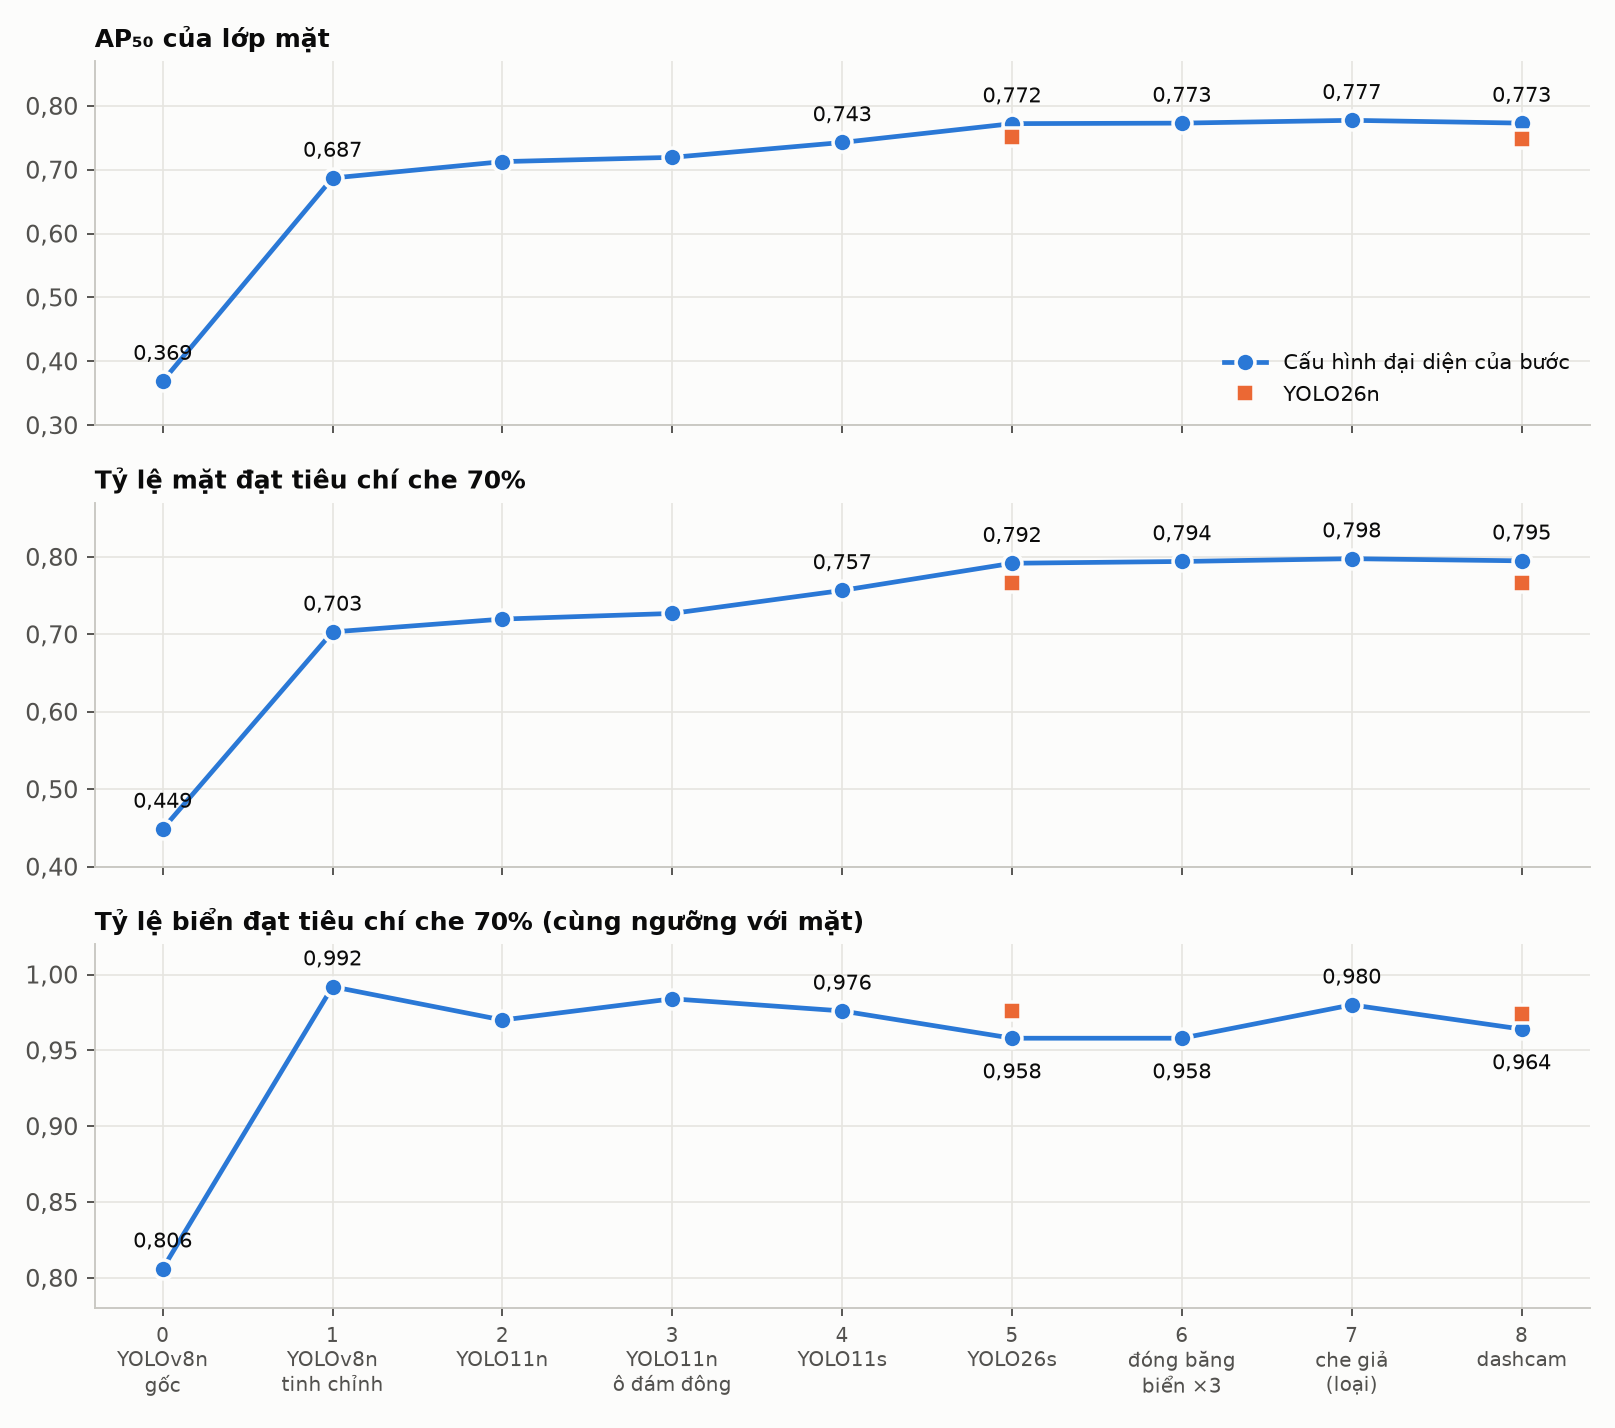
\includegraphics[width=0.8\textwidth]{figures/hinh-4-2-hanh-trinh.png}
\caption[Face AP và tỷ lệ che qua các bước huấn luyện]{Face AP và tỷ lệ che qua các bước huấn luyện, mỗi bước lấy một cấu hình đại diện. Điểm vuông là YOLO26n}
\label{fig:4-2}
\end{figure}

\textbf{Bước 0 và 1.} Mô hình gốc chỉ đạt 0,449 mặt được che. Sau 10 epoch huấn luyện trên WIDER và biển số Việt Nam, con số này lên 0,700, còn biển tăng từ 0,806 lên 0,960. Đây là bước cải thiện lớn nhất, cho thấy dữ liệu đúng bài toán quan trọng hơn mọi mẹo về sau.

\textbf{Bước 2.} YOLO11n với cùng dữ liệu tốt hơn YOLOv8n ở cả AP (0,713 so với 0,687) và tỷ lệ mặt được che (0,720 so với 0,703). Nhóm cũng thử cùng bộ trọng số ở ba kích thước đầu vào (Bảng~\ref{tab:4-3}). Chạy ở 640 px làm mất 21 điểm phần trăm, nhiều hơn hẳn lợi ích của việc đổi sang mô hình lớn hơn, vì vậy Engine mặc định dùng 1280 px.

\begin{table}[!htp]
\centering\bangfont
\caption{Độ chính xác theo kích thước đầu vào 640 / 960 / 1280}\label{tab:4-3}
\begin{tabular}{|L{2.9cm}|L{3.1cm}|C{1.2cm}|C{1.2cm}|C{1.2cm}|L{4.4cm}|}
\hline
\dongdau \textbf{Mô hình} & \textbf{Chỉ số} & \textbf{640} & \textbf{960} & \textbf{1280} & \textbf{Nhận xét} \\ \hline
YOLO11n, 20 epoch & Face AP & 0,519 & 0,650 & 0,713 & Cùng precision mặt 0,78 \\ \cline{2-6}
 & Mặt đạt che & 0,510 & 0,653 & 0,720 & Mất 6,7 điểm ở 960, 21 điểm ở 640 \\ \cline{2-6}
 & Mặt < 16 px đạt che & 0,202 & 0,427 & 0,541 & Mặt nhỏ mất nhiều nhất \\ \hline
YOLOv8n gốc & Face AP & 0,219 & 0,306 & 0,369 & Precision 0,794--0,811, chỉ so trong cùng hàng \\ \cline{2-6}
 & Mặt đạt che & 0,307 & 0,377 & 0,449 & Tăng kích thước vẫn kém mô hình đã tinh chỉnh \\ \hline
\end{tabular}
\end{table}

\textbf{Bước 3.} Nhóm thử ba mẹo về dữ liệu. Thêm nhãn giả làm kết quả giảm nhẹ (0,713) nên bị loại. Cắt ảnh đám đông thành ô đưa tỷ lệ lên 0,727 và được giữ lại. Lặp thêm ảnh mặt nhỏ chỉ tăng 0,001 trong khi AP giảm, nên cũng bỏ.

\textbf{Bước 4 và 5.} YOLO11s lúc đầu chỉ huấn luyện 12 epoch nên chưa so được công bằng. Ở bước 5 nhóm thống nhất công thức: 1280 px, 20 epoch, có ô đám đông. YOLO26n đạt 0,766 so với 0,749 của YOLO11n, còn YOLO26s đạt 0,792 nhưng tỷ lệ biển lại giảm từ 0,984 (YOLO26n) xuống 0,960. Nhóm chưa chạy lại YOLO11s với công thức này.

\textbf{Bước 6.} Để lấy lại biển số cho YOLO26s, thử nghiệm đầu tiên huấn luyện thêm bằng AdamW nhưng biển còn giảm xuống 0,950. Nhóm quay lại mô hình 20 epoch, đóng băng backbone, dùng SGD và lặp ảnh biển hai lần. AP biển tăng từ 0,963 lên 0,980 mà mặt gần như không đổi. Thêm 5 epoch với ảnh biển lặp ba lần đưa tỷ lệ biển lên 0,974. Vì ba yếu tố thay đổi cùng lúc nên nhóm không kết luận yếu tố nào quyết định.

\textbf{Bước 7.} Khi đánh giá trên video, nhóm phát hiện biển bị che một phần bị bỏ sót tới 55,7\%. Kiểm tra ngẫu nhiên 120 biển trong tập huấn luyện thì không có biển nào bị che. Nhóm dán mảnh ảnh che 25--70\% biển để tạo thêm mẫu. Trên ảnh, tỷ lệ biển tăng lên 0,980, nhưng trên video mức bỏ sót chỉ giảm xuống 52,5\%, trong khi tỷ lệ giữ đúng biển chủ xe giảm từ 87,1\% xuống 77,0\% và số khung người lạ bị giữ nhầm tăng từ 2 lên 10. Cả hai biến thể đều bị loại.

\textbf{Bước 8.} Từ mô hình của từng chế độ, nhóm huấn luyện thêm 5 epoch với 468 khung dashcam lặp bốn lần, vẫn giữ dữ liệu cũ và đóng băng backbone. Trên bộ đánh giá ảnh, mặt gần như không đổi (0,766 lên 0,767 và 0,794 lên 0,795), nhưng tỷ lệ biển ở điểm D giảm từ 0,984 xuống 0,970 (YOLO26n) và từ 0,974 xuống 0,948 (YOLO26s). Một phần do bộ đánh giá chỉ gán nhãn một biển chính mỗi ảnh: xem ngẫu nhiên 24 hộp bị tính là sai thì khoảng 18--20 hộp là biển thật của xe phía sau. Lợi ích của bước này chỉ thấy rõ trên video (mục 4.8), và đó là lý do nhóm chọn. Biến thể thêm ảnh đồng hồ xe làm mẫu âm bị loại vì với YOLO26n, tỷ lệ giữ đúng biển chủ xe trên clip dashcam 2 giảm từ 83,8\% xuống 52,9\%.

\textbf{Quá trình huấn luyện hai mô hình được chọn.} Trên tập validation, YOLO26s đạt mAP\textsubscript{50} 0,914 và YOLO26n đạt 0,903 ở epoch cuối (Hình~\ref{fig:4-3} và~\ref{fig:4-4}). Trên bộ đánh giá, mAP\textsubscript{50} của hai mô hình là 0,870 và 0,865. Hai loại số này đo trên dữ liệu khác nhau nên không đặt cạnh nhau. Tập validation không có khung dashcam nên không phản ánh lợi ích của bước 8, vì vậy nhóm dùng trọng số của epoch cuối thay vì epoch có validation cao nhất.

\begin{figure}[!htp]
\centering
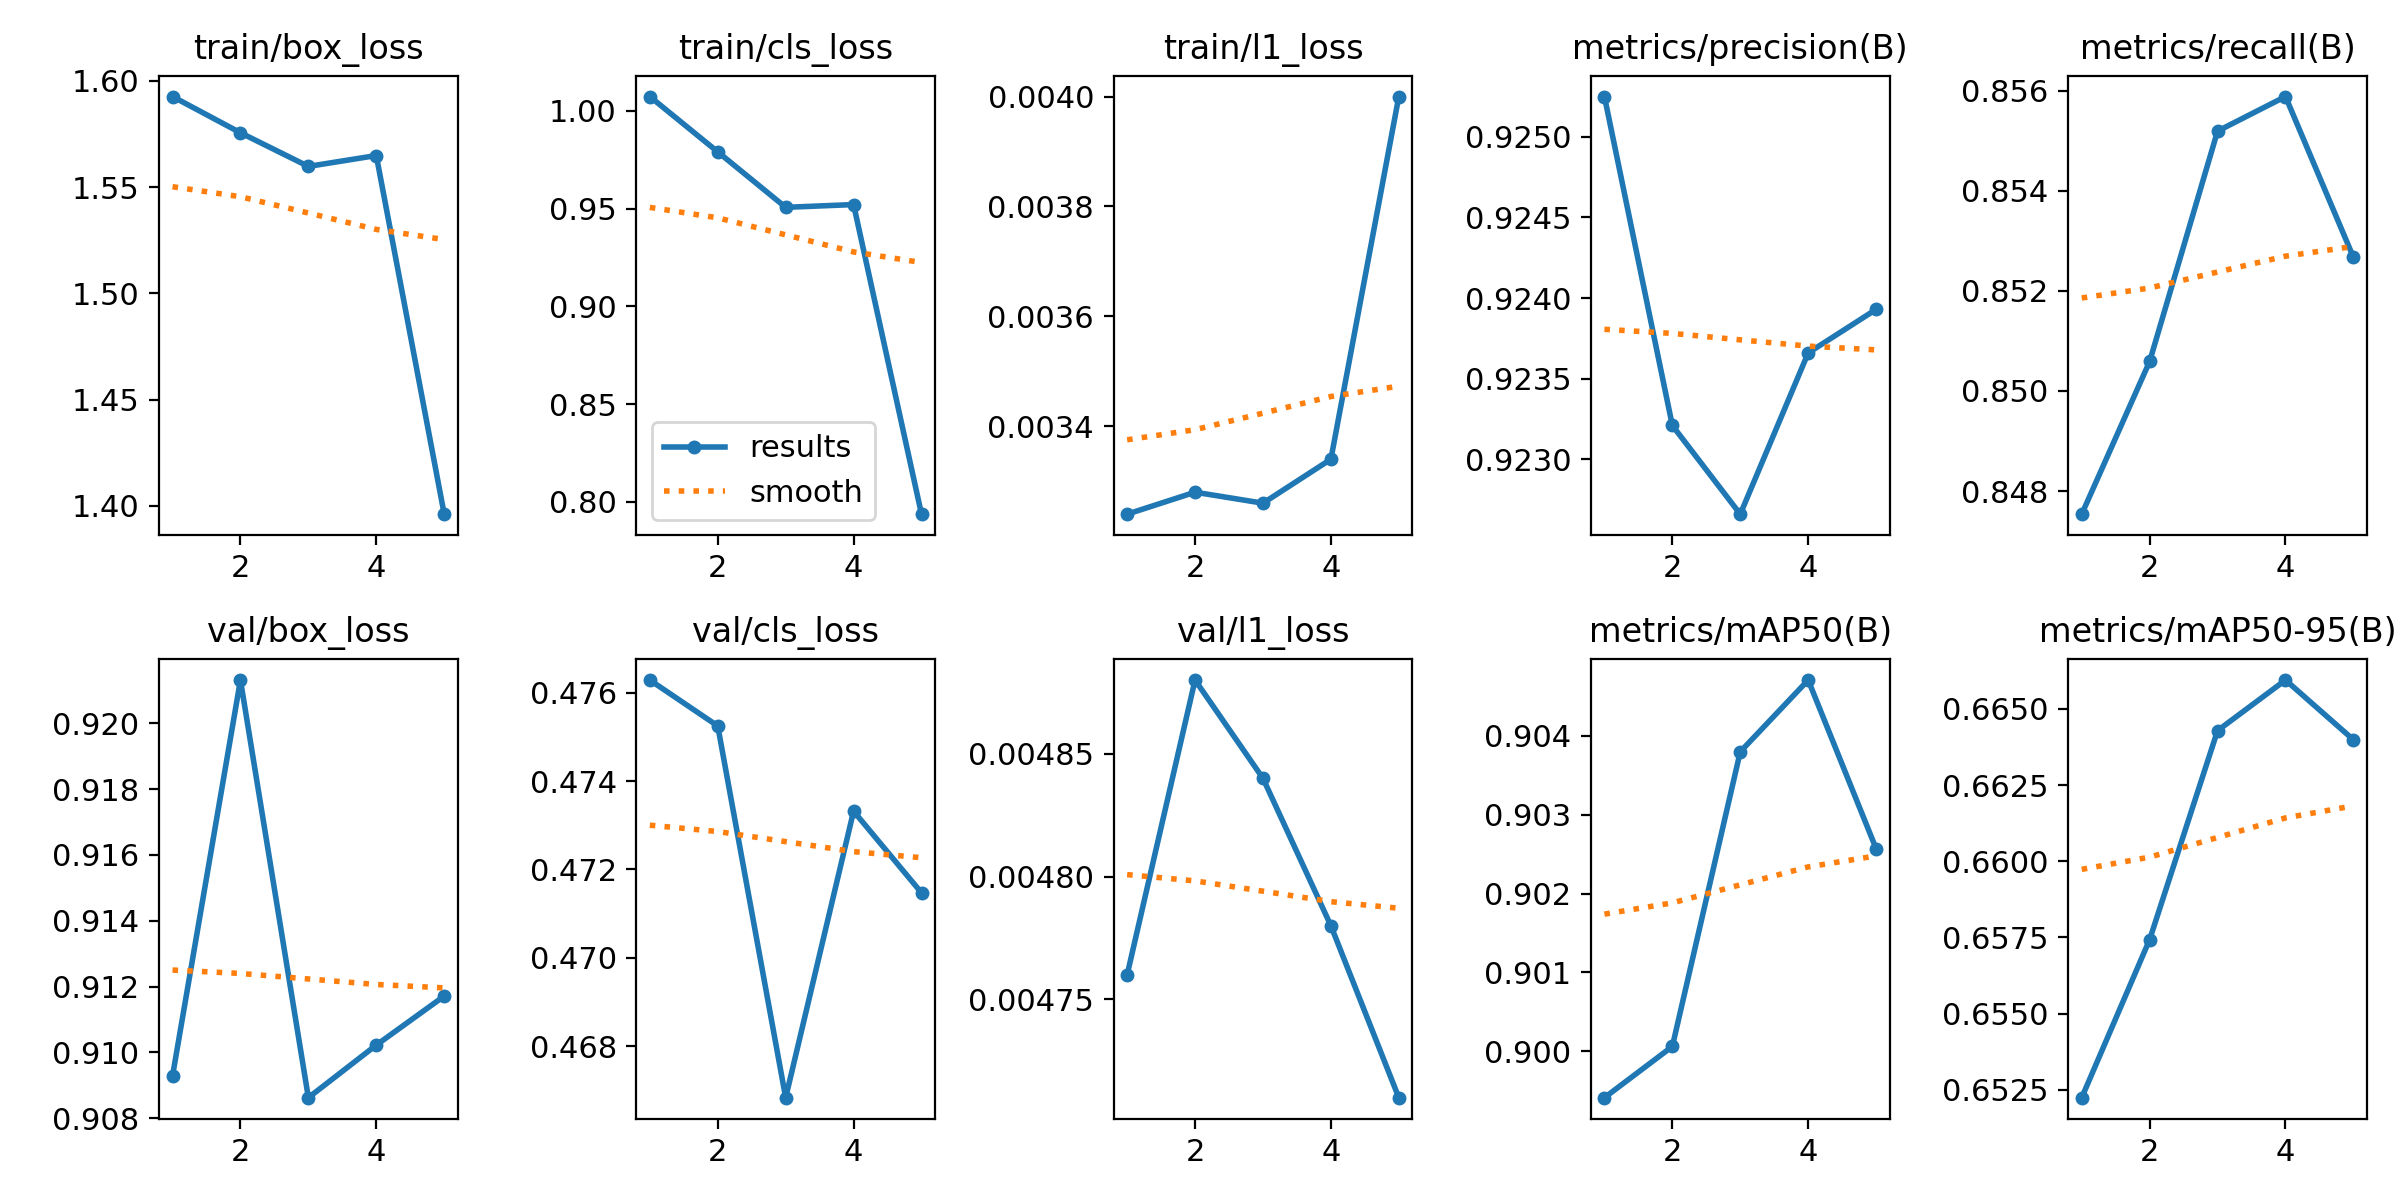
\includegraphics[width=0.98\textwidth]{figures/hinh-4-3-results-yolo26n.png}
\caption[Đường cong huấn luyện của YOLO26n (chế độ Fast)]{Đường cong huấn luyện của YOLO26n e5-dashcam (chế độ Fast), đo trên validation}
\label{fig:4-3}
\end{figure}

\begin{figure}[!htp]
\centering
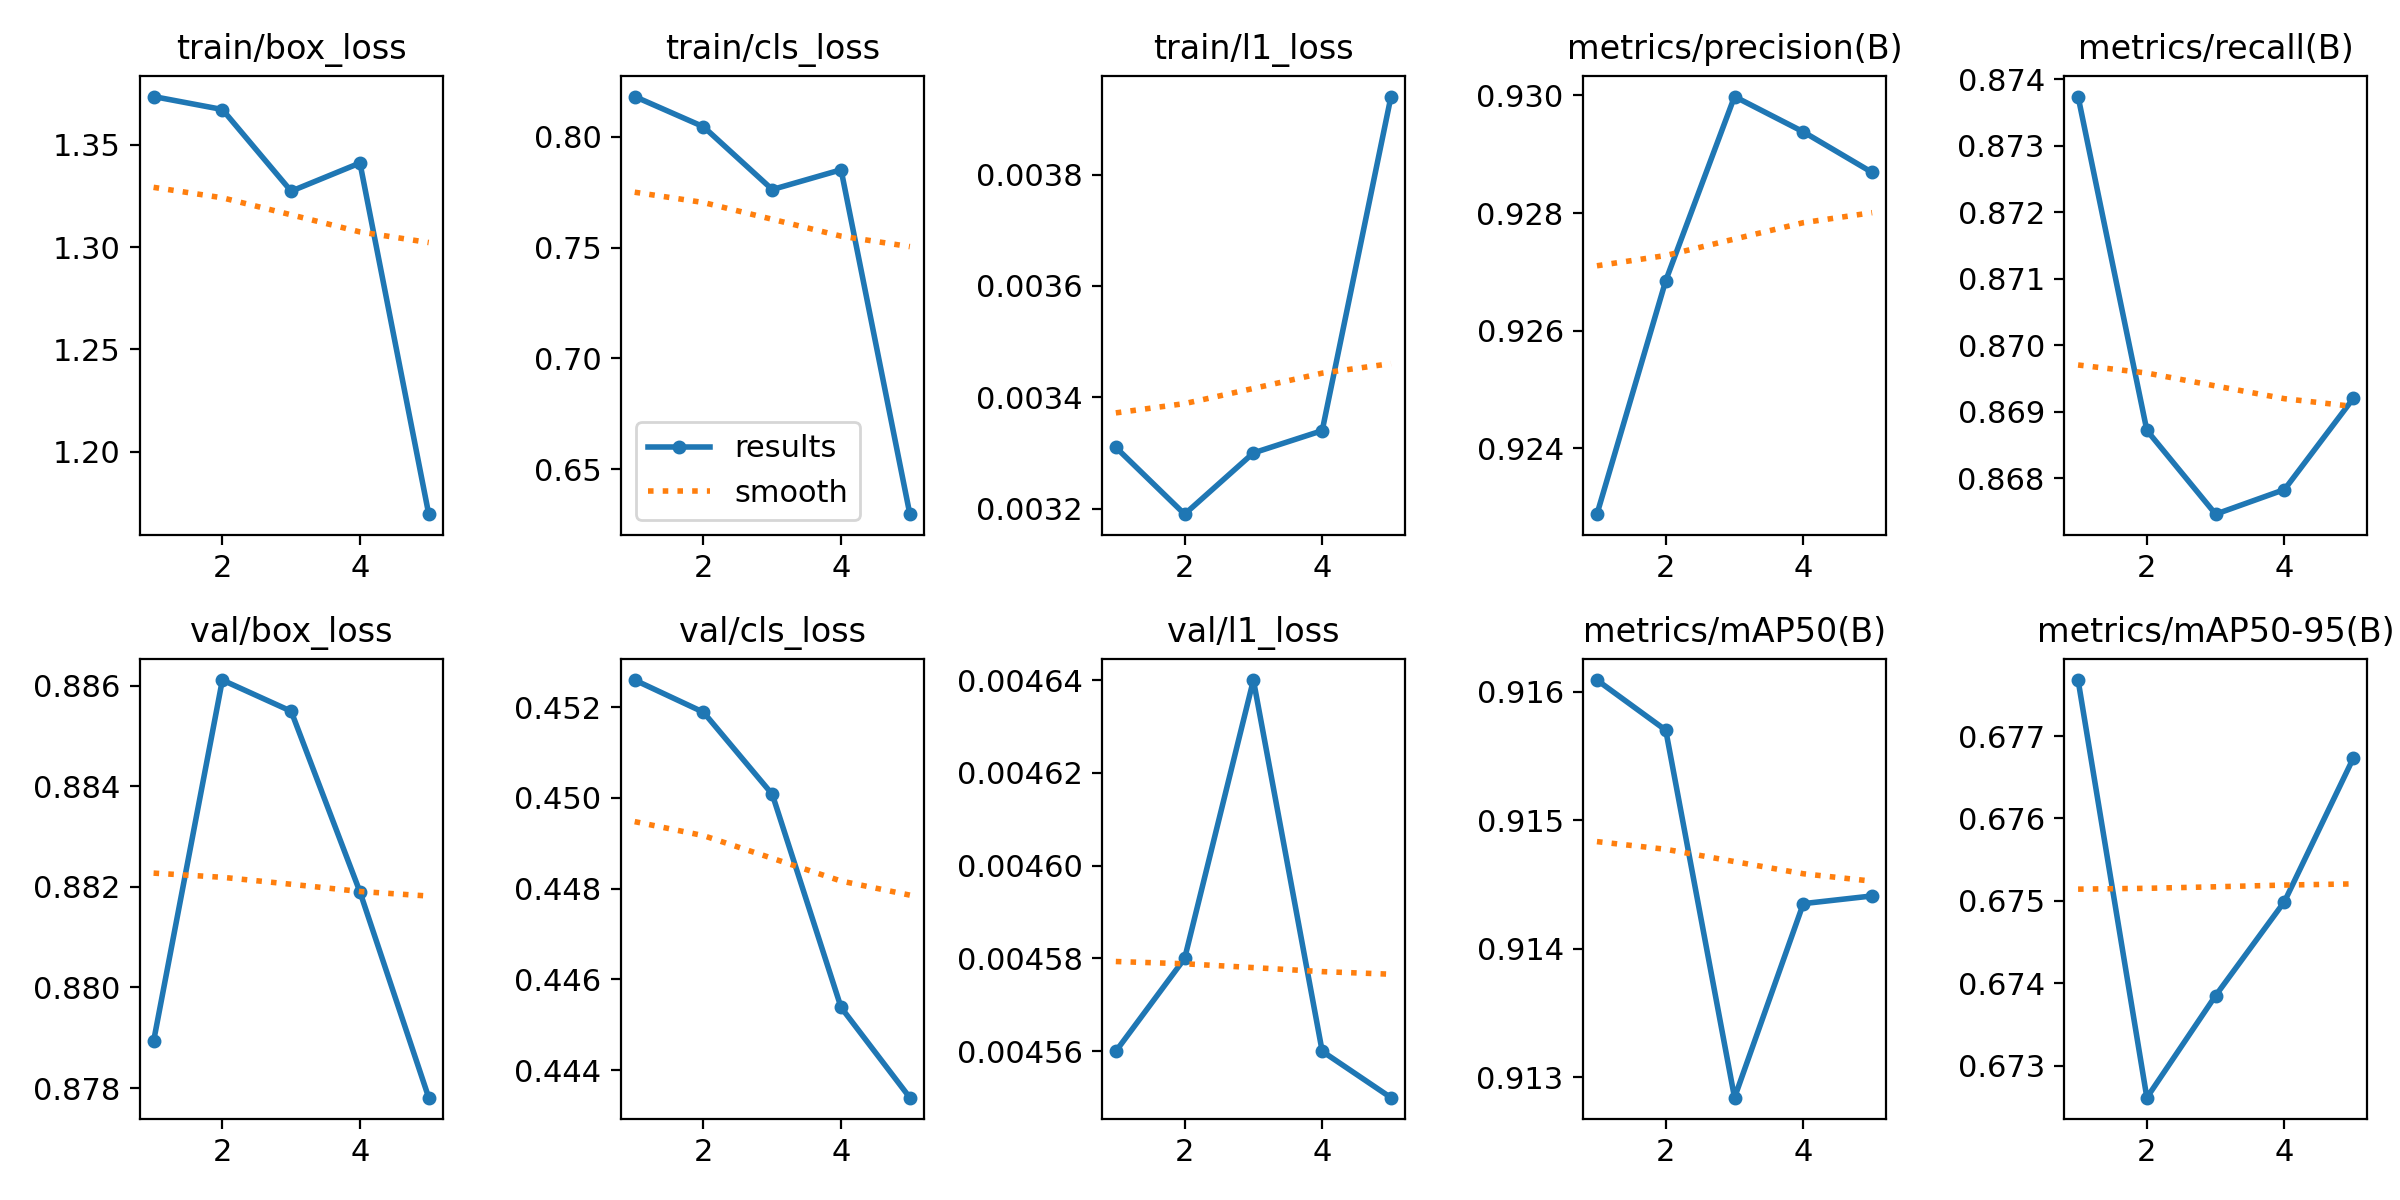
\includegraphics[width=0.98\textwidth]{figures/hinh-4-4-results-yolo26s.png}
\caption[Đường cong huấn luyện của YOLO26s (chế độ Maximum privacy)]{Đường cong huấn luyện của YOLO26s e5-dashcam (chế độ Maximum privacy), đo trên validation}
\label{fig:4-4}
\end{figure}

Hình~\ref{fig:4-5} đến~\ref{fig:4-7} cho thấy lớp biển dễ hơn lớp mặt: biển giữ $F_1$ cao trên một dải ngưỡng rộng, còn mặt giảm nhanh khi ngưỡng vượt 0,4. $F_1$ đạt đỉnh ở ngưỡng khoảng 0,31 (YOLO26n) và 0,33 (YOLO26s), nhưng Engine dùng ngưỡng thấp hơn để giảm bỏ sót. Ở ma trận nhầm lẫn, hai lớp hầu như không lẫn nhau, hộp sai chủ yếu là nền bị nhận thành mặt.

\begin{figure}[!htp]
\centering
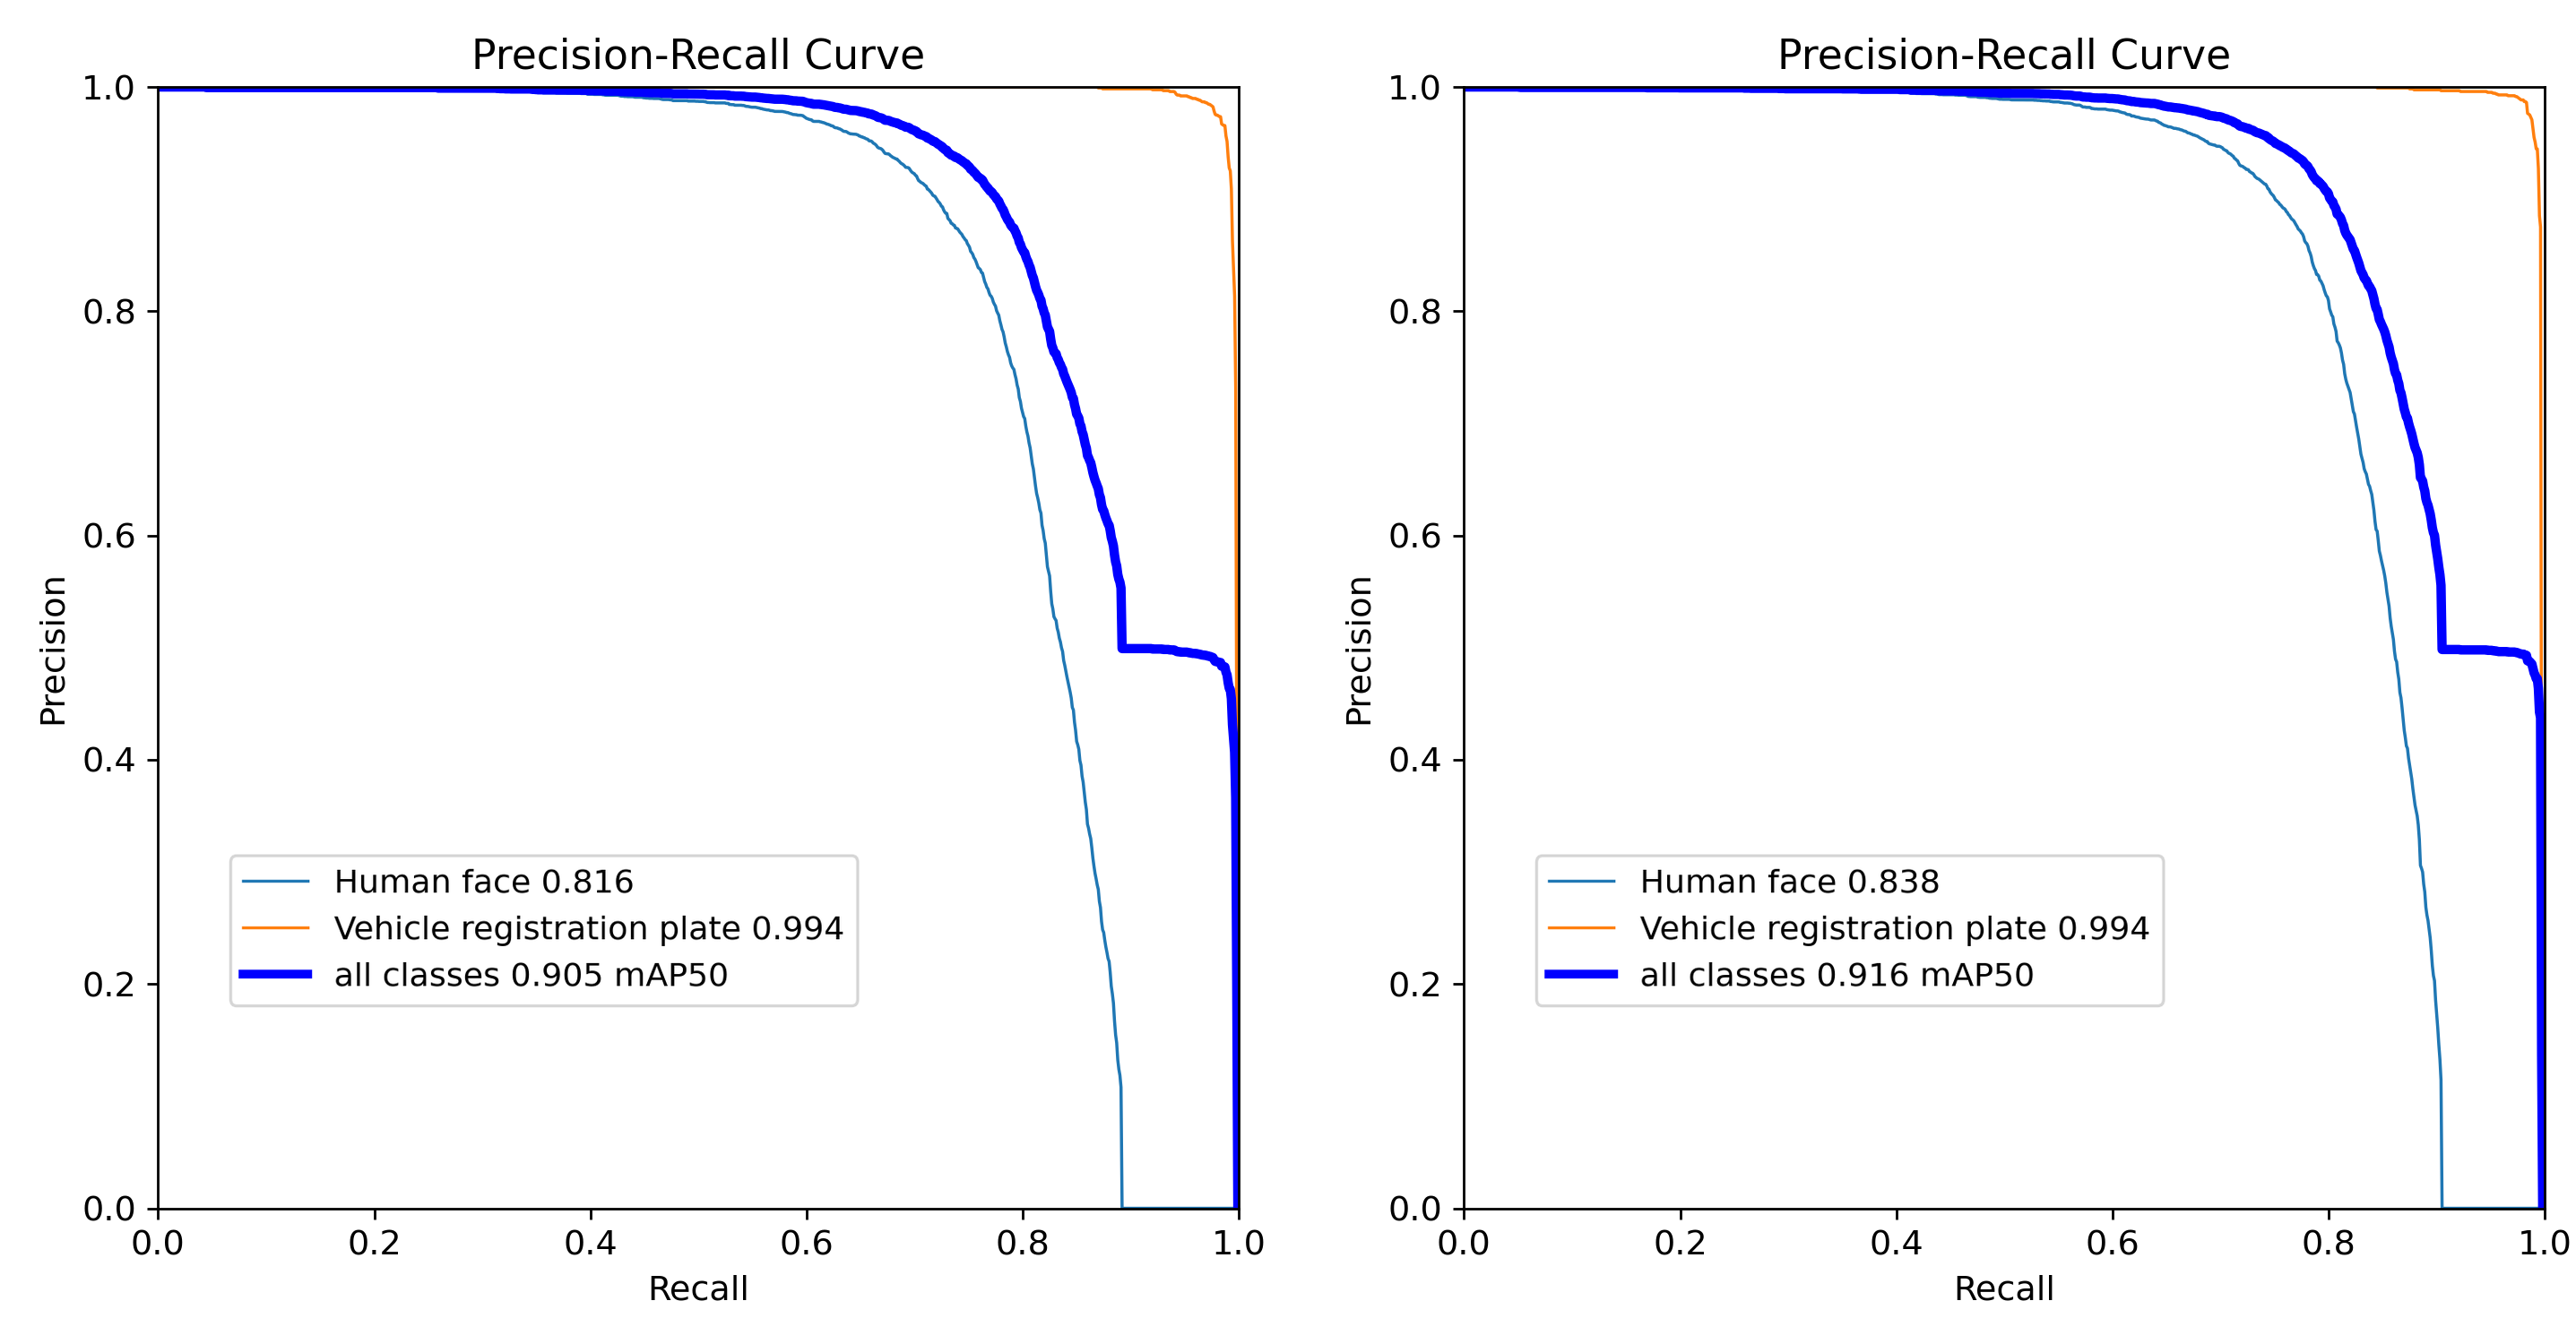
\includegraphics[width=0.98\textwidth]{figures/hinh-4-5-pr.png}
\caption[Đường cong Precision--Recall của hai mô hình được chọn]{Đường Precision--Recall của YOLO26n (trái) và YOLO26s (phải) trên validation}
\label{fig:4-5}
\end{figure}

\begin{figure}[!htp]
\centering
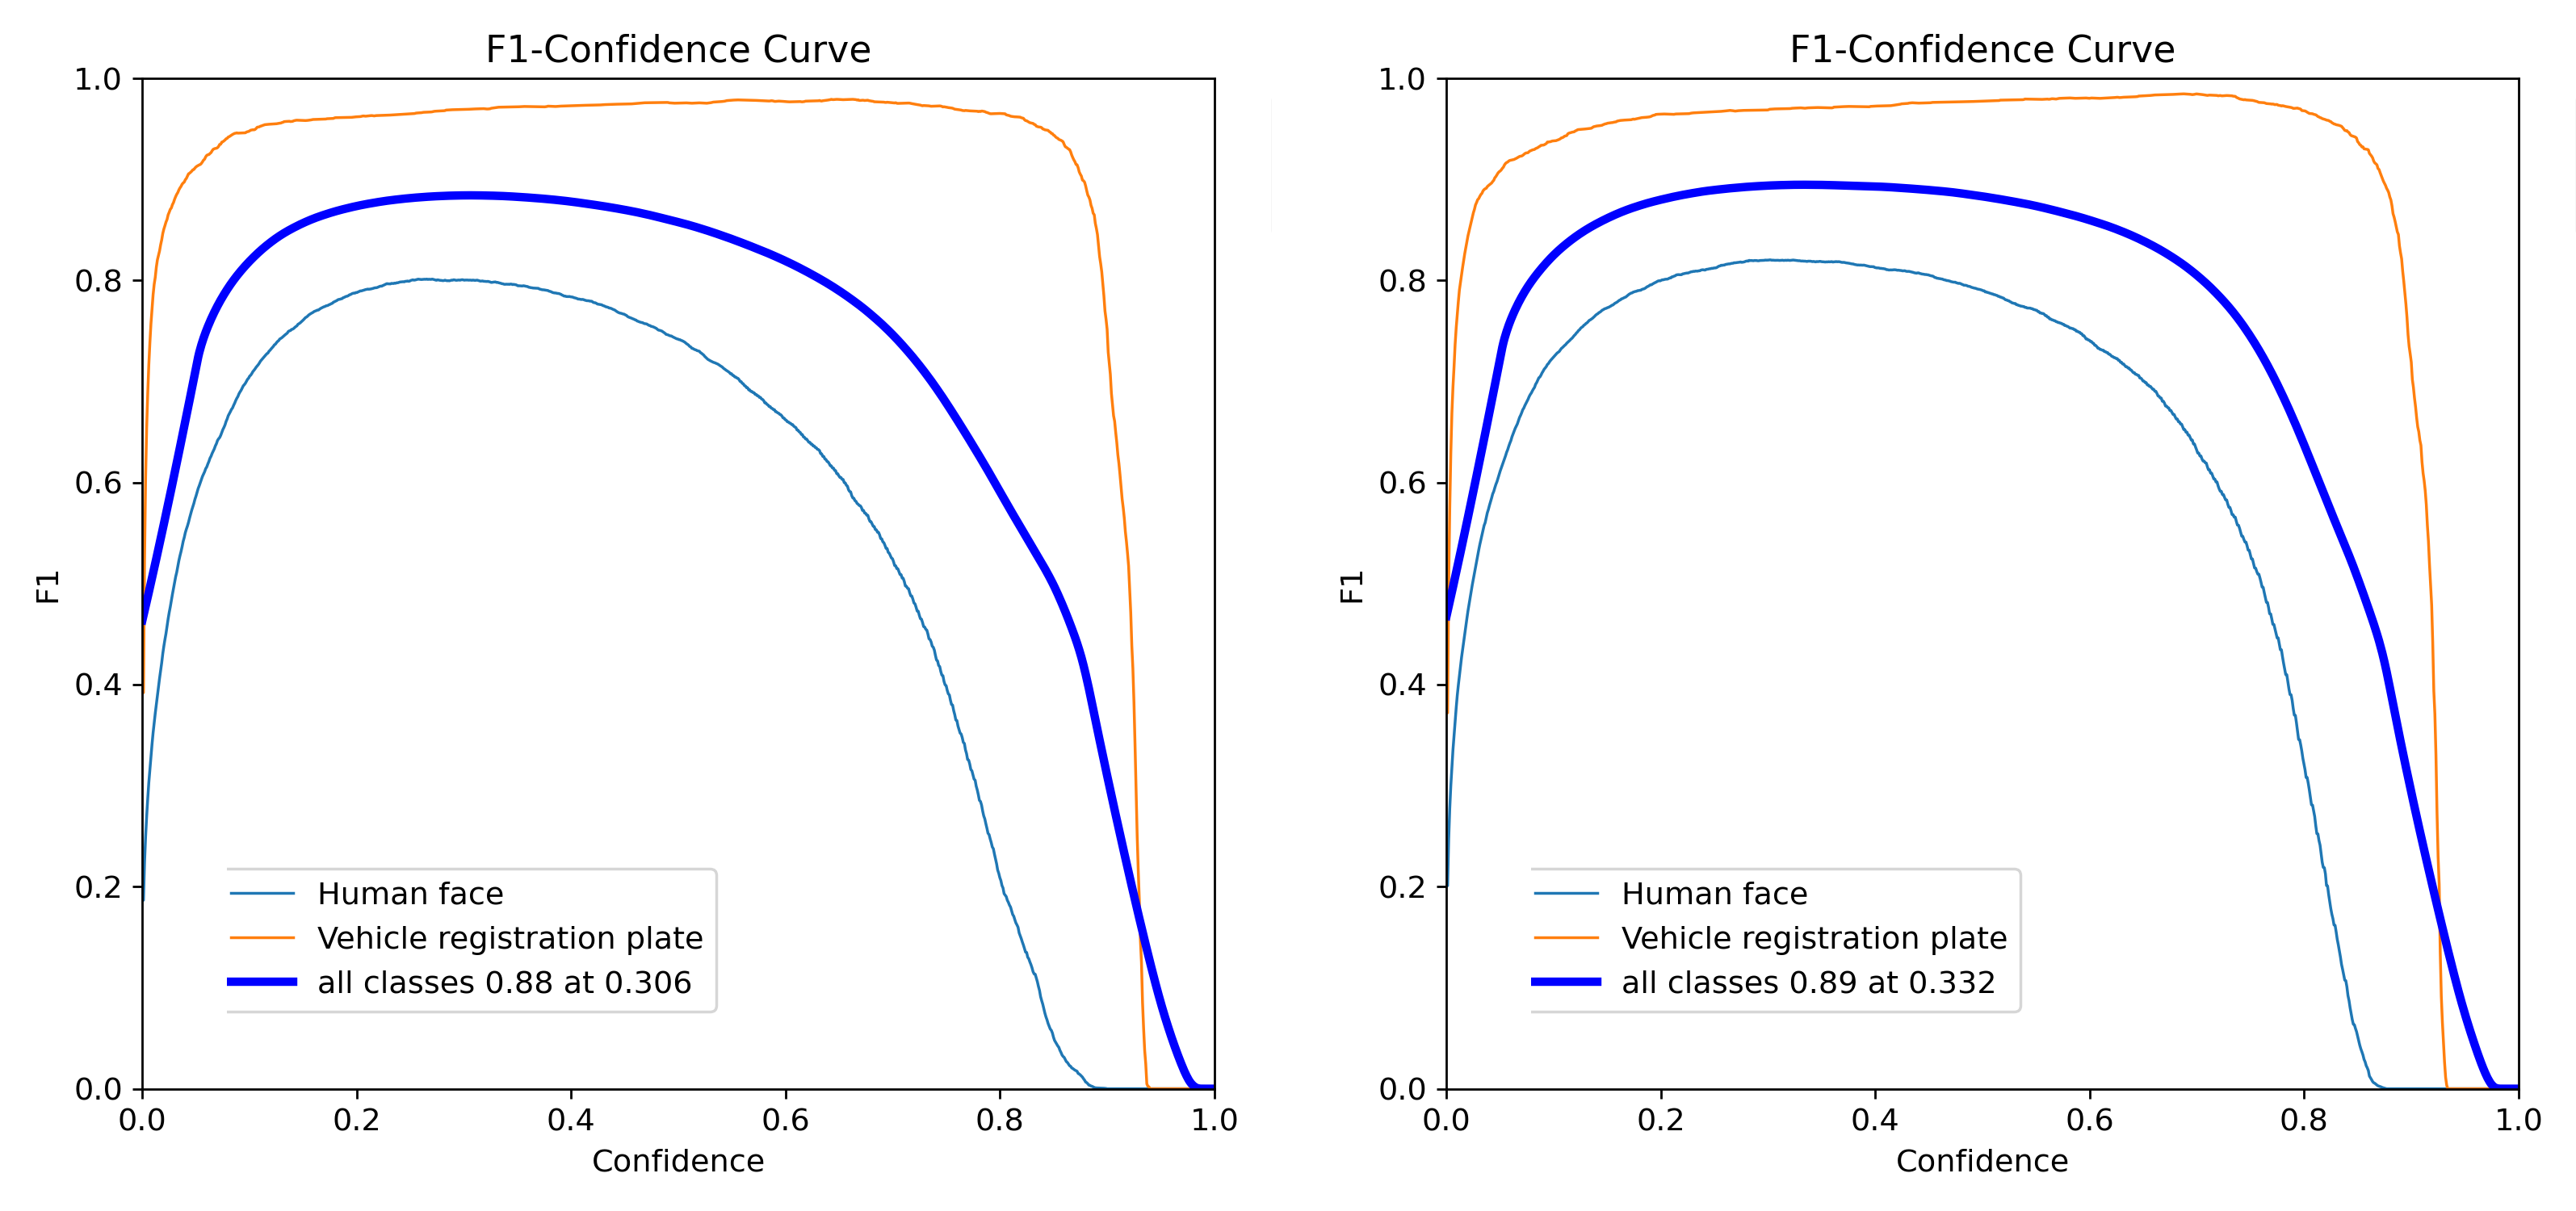
\includegraphics[width=0.98\textwidth]{figures/hinh-4-6-f1.png}
\caption[Đường cong $F_1$ theo ngưỡng tin cậy]{Đường $F_1$ theo ngưỡng tin cậy của YOLO26n (trái) và YOLO26s (phải)}
\label{fig:4-6}
\end{figure}

\begin{figure}[!htp]
\centering
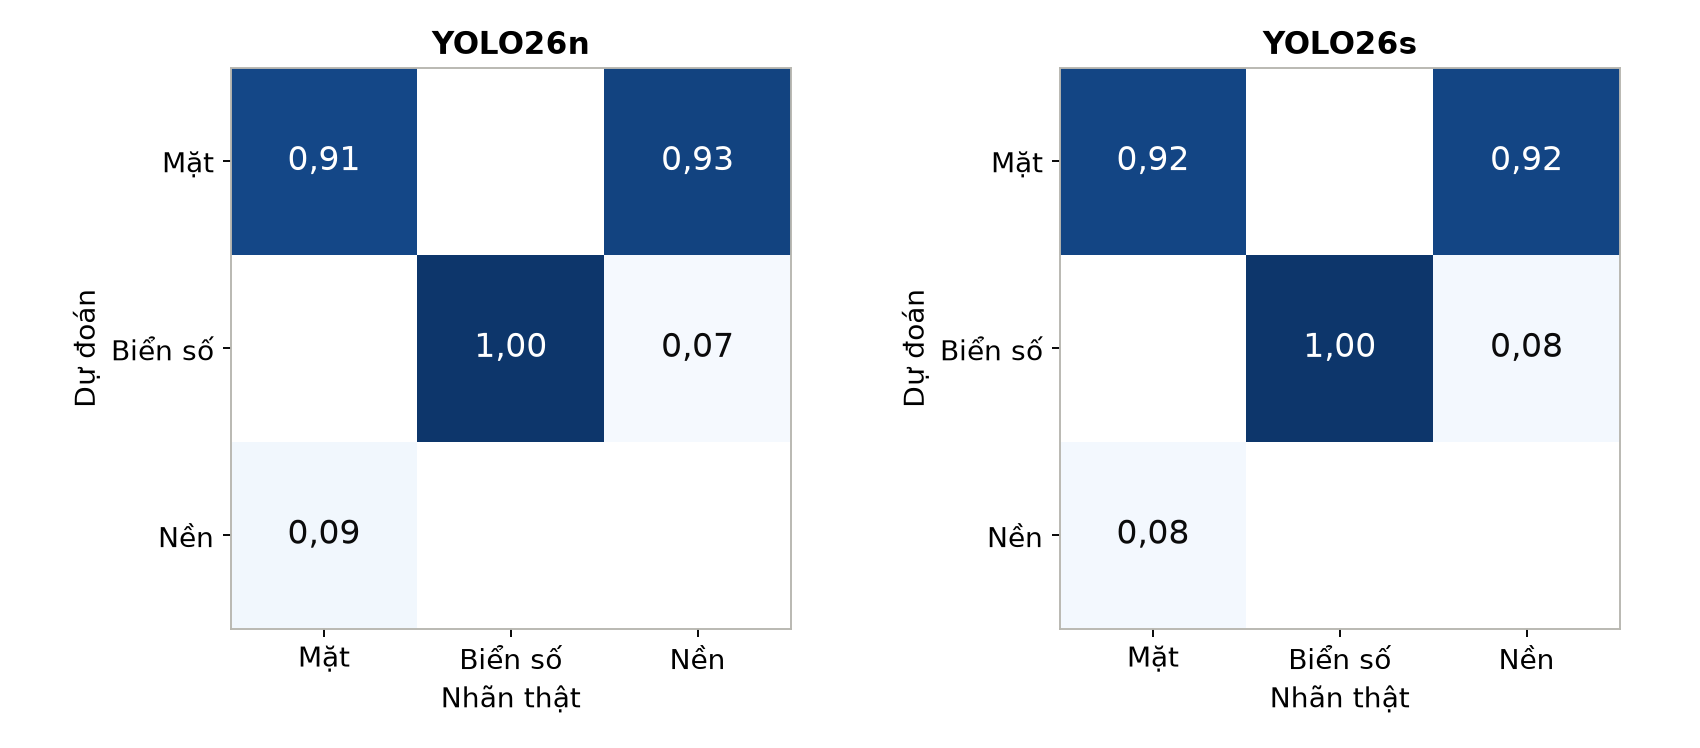
\includegraphics[width=0.98\textwidth]{figures/hinh-4-7-ma-tran.png}
\caption[Ma trận nhầm lẫn chuẩn hoá]{Ma trận nhầm lẫn chuẩn hoá của YOLO26n (trái) và YOLO26s (phải) trên validation}
\label{fig:4-7}
\end{figure}

\begin{figure}[!htp]
\centering
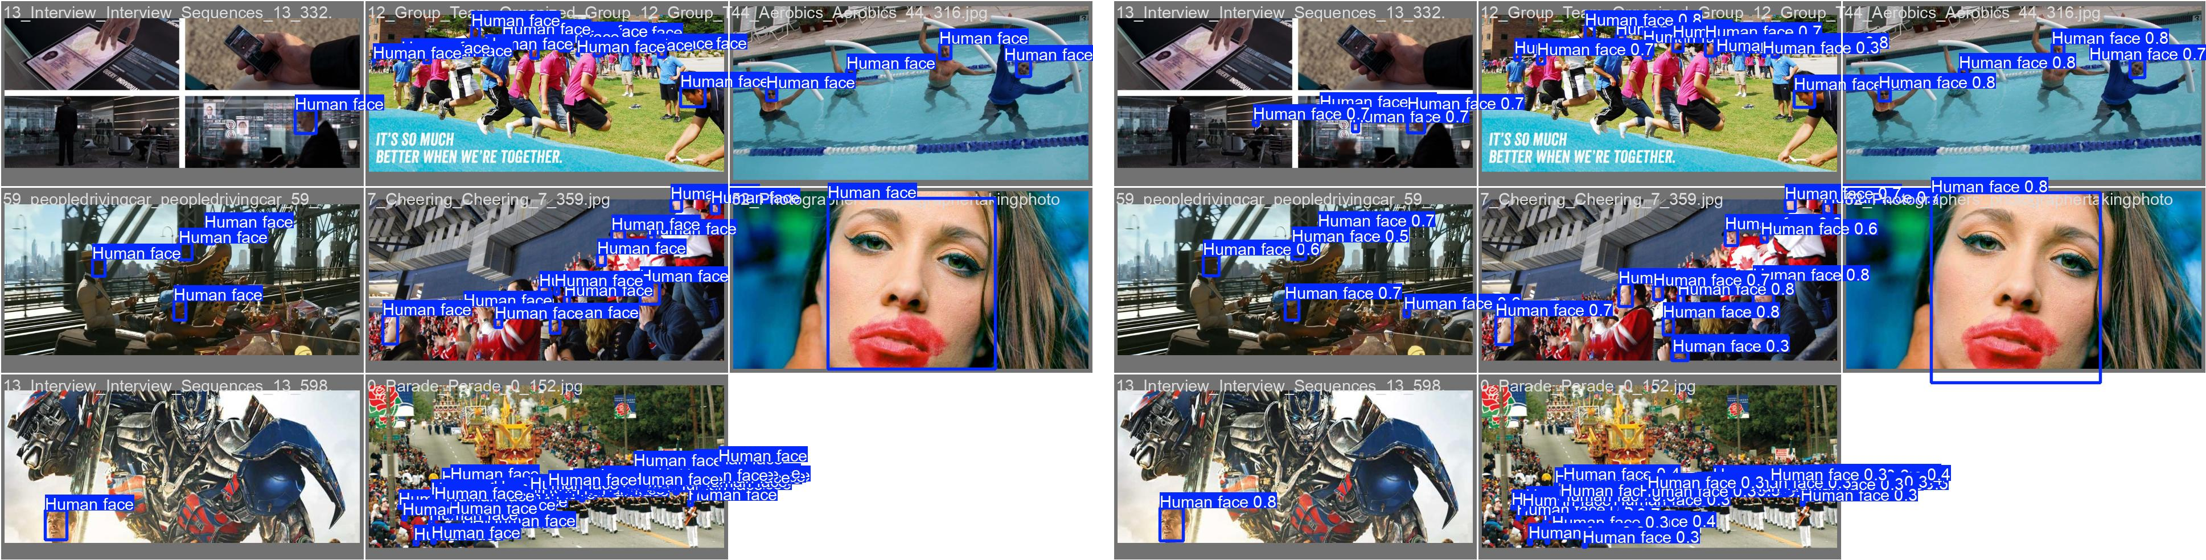
\includegraphics[width=0.98\textwidth]{figures/hinh-4-8-nhan-du-doan.png}\\[4pt]
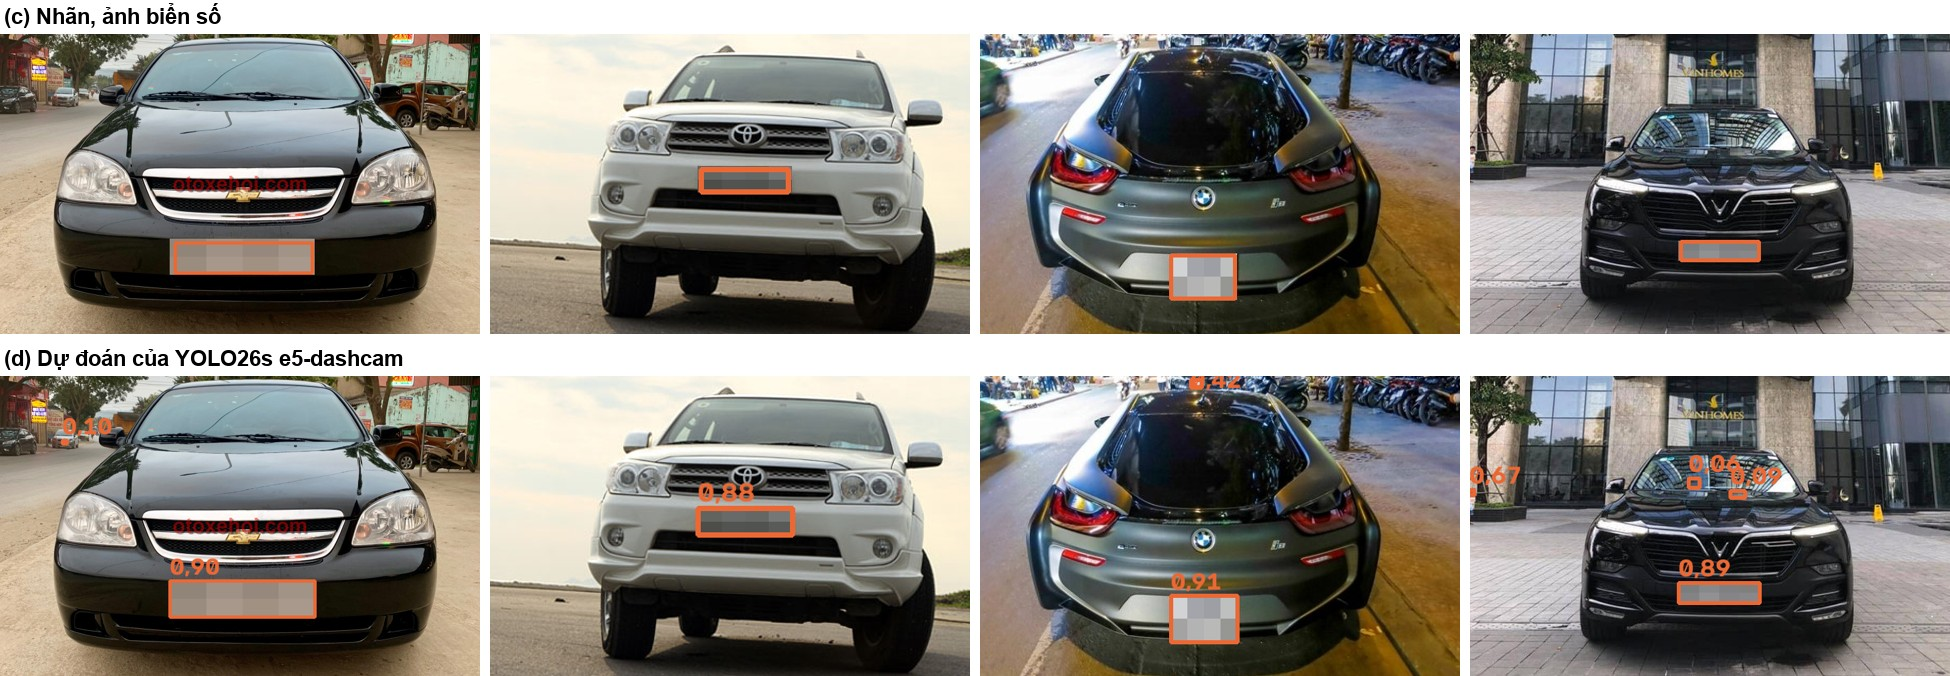
\includegraphics[width=0.98\textwidth]{figures/hinh-4-8-bien-so.jpg}
\caption[So sánh nhãn và dự đoán]{So sánh nhãn và dự đoán của YOLO26s e5-dashcam. Trên: một batch validation của WIDER FACE, trái là nhãn, phải là dự đoán. Dưới: bốn ảnh biển số của bộ đánh giá, vùng biển được làm mờ khi in}
\label{fig:4-8}
\end{figure}

\subsection{Chế độ phát hiện và ngưỡng theo từng lớp}

Người dùng chọn một trong hai chế độ. Fast dùng YOLO26n, hợp với việc duyệt nhanh. Maximum privacy dùng YOLO26s với ngưỡng thấp hơn, ưu tiên giảm bỏ sót. Bảng~\ref{tab:4-4} ghi kết quả ở đúng ngưỡng triển khai.

\begin{table}[!htp]
\centering\bangfont
\caption{Cấu hình các chế độ phát hiện}\label{tab:4-4}
\begin{tabular}{|L{6.0cm}|C{4.4cm}|C{4.4cm}|}
\hline
\dongdau & \textbf{Fast} & \textbf{Maximum privacy} \\ \hline
Mô hình & YOLO26n e5-dashcam & YOLO26s e5-dashcam \\ \hline
Kích thước đầu vào & 1280 px & 1280 px \\ \hline
Ngưỡng mặt / biển & 0,17 / 0,11 & 0,06 / 0,05 \\ \hline
Mặt: precision / recall & 0,797 / 0,726 & 0,608 / 0,797 \\ \hline
Mặt đạt che: tất cả / $\ge$16 px / <16 px & 0,761 / 0,910 / 0,606 & 0,834 / 0,950 / 0,714 \\ \hline
Biển: precision / recall & 0,747 / 0,980 & 0,643 / 0,978 \\ \hline
Số mặt không đạt che & khoảng 9.350 & khoảng 6.480 \\ \hline
Số hộp mặt sai & khoảng 7.200 & khoảng 20.100 \\ \hline
Tốc độ, GPU RTX 3050 (p50 mỗi ảnh) & 61--65 ms & 102--104 ms \\ \hline
Tốc độ, CPU i5-7200U (p50 mỗi ảnh) & 0,96--1,20 s & 2,85--2,99 s \\ \hline
Khi nào dùng & Duyệt nhanh, chấp nhận sót một số mặt nhỏ & Ưu tiên không bỏ sót, chấp nhận che nhầm nhiều hơn \\ \hline
\end{tabular}
\end{table}

\textbf{Ngưỡng riêng cho từng lớp.} Biển thường có điểm thấp hơn mặt. Với YOLO26n, nếu dùng chung ngưỡng 0,17 thì tỷ lệ biển đạt che là 0,974, còn hạ riêng ngưỡng biển xuống 0,11 thì lên 0,980, đổi lại precision biển giảm từ 0,796 xuống 0,747.

\textbf{Đánh đổi giữa hai chế độ.} Chuyển từ Fast sang Max privacy giảm khoảng 2.870 mặt không được che, chủ yếu là mặt dưới 16 px, nhưng số hộp mặt sai tăng gần ba lần. Một phần hộp sai là mặt mờ mà WIDER không gán nhãn. Với biển cận cảnh, hai chế độ gần như ngang nhau, lợi thế của Max privacy chỉ rõ trên video dashcam. Nhóm cũng thử đặt ngưỡng theo kích thước mặt: hạ ngưỡng cho mặt nhỏ tìm thêm 890 mặt nhưng kéo theo 5.619 hộp sai, nên cuối cùng chỉ giữ ngưỡng theo lớp và theo chế độ.

\subsection{So sánh với các công cụ mã nguồn mở}

Nhóm so với ba công cụ có mô hình mở: deface (dùng CenterFace, chỉ che mặt), YuNet của OpenCV (Wu và cộng sự, 2023) và EgoBlur Gen2 của Meta (Raina và cộng sự, 2023), gồm hai mô hình riêng cho mặt và biển. Bảng~\ref{tab:4-5} chỉ đặt cạnh nhau những phép đo trên cùng tập ảnh, cùng cách chấm và cùng precision mặt.

\begin{table}[!htp]
\centering\bangfont
\caption[So sánh độ chính xác với deface, YuNet, EgoBlur]{So sánh độ chính xác với deface, YuNet, EgoBlur trên bộ đánh giá 3.726 ảnh}\label{tab:4-5}
\begin{tabular}{|L{3.7cm}|C{1.6cm}|C{2.1cm}|C{2.1cm}|C{2.1cm}|C{2.1cm}|}
\hline
\dongdau \textbf{Công cụ / mô hình} & \textbf{Face AP} & \textbf{Mặt đạt che, P 0,781} & \textbf{Mặt đạt che, P 0,643} & \textbf{Mặt $\ge$16 px, P 0,781} & \textbf{Biển đạt che, P $\ge$ 0,90} \\ \hline
Max privacy (YOLO26s) & \textbf{0,773} & \textbf{0,795} & \textbf{0,828} & \textbf{0,931} & 0,948 \\ \hline
Fast (YOLO26n) & 0,748 & 0,767 & 0,803 & 0,913 & 0,970 \\ \hline
YuNet & 0,651 & 0,670 & 0,737 & 0,860 & không có \\ \hline
deface, toàn ảnh & 0,649 & 0,663 & 0,723 & 0,909 & không có \\ \hline
deface, 640$\times$480 & 0,471 & 0,490 & 0,538 & 0,825 & không có \\ \hline
EgoBlur Gen2* & 0,534 & 0,572 & --- & 0,835 & \textbf{1,000} \\ \hline
\end{tabular}
\par\vspace{3pt}{\noindent\small\itshape * Precision thấp nhất đạt được là 0,816 nên hai cột mặt của EgoBlur đo ở mức này.\par}
\end{table}

\begin{figure}[!htp]
\centering
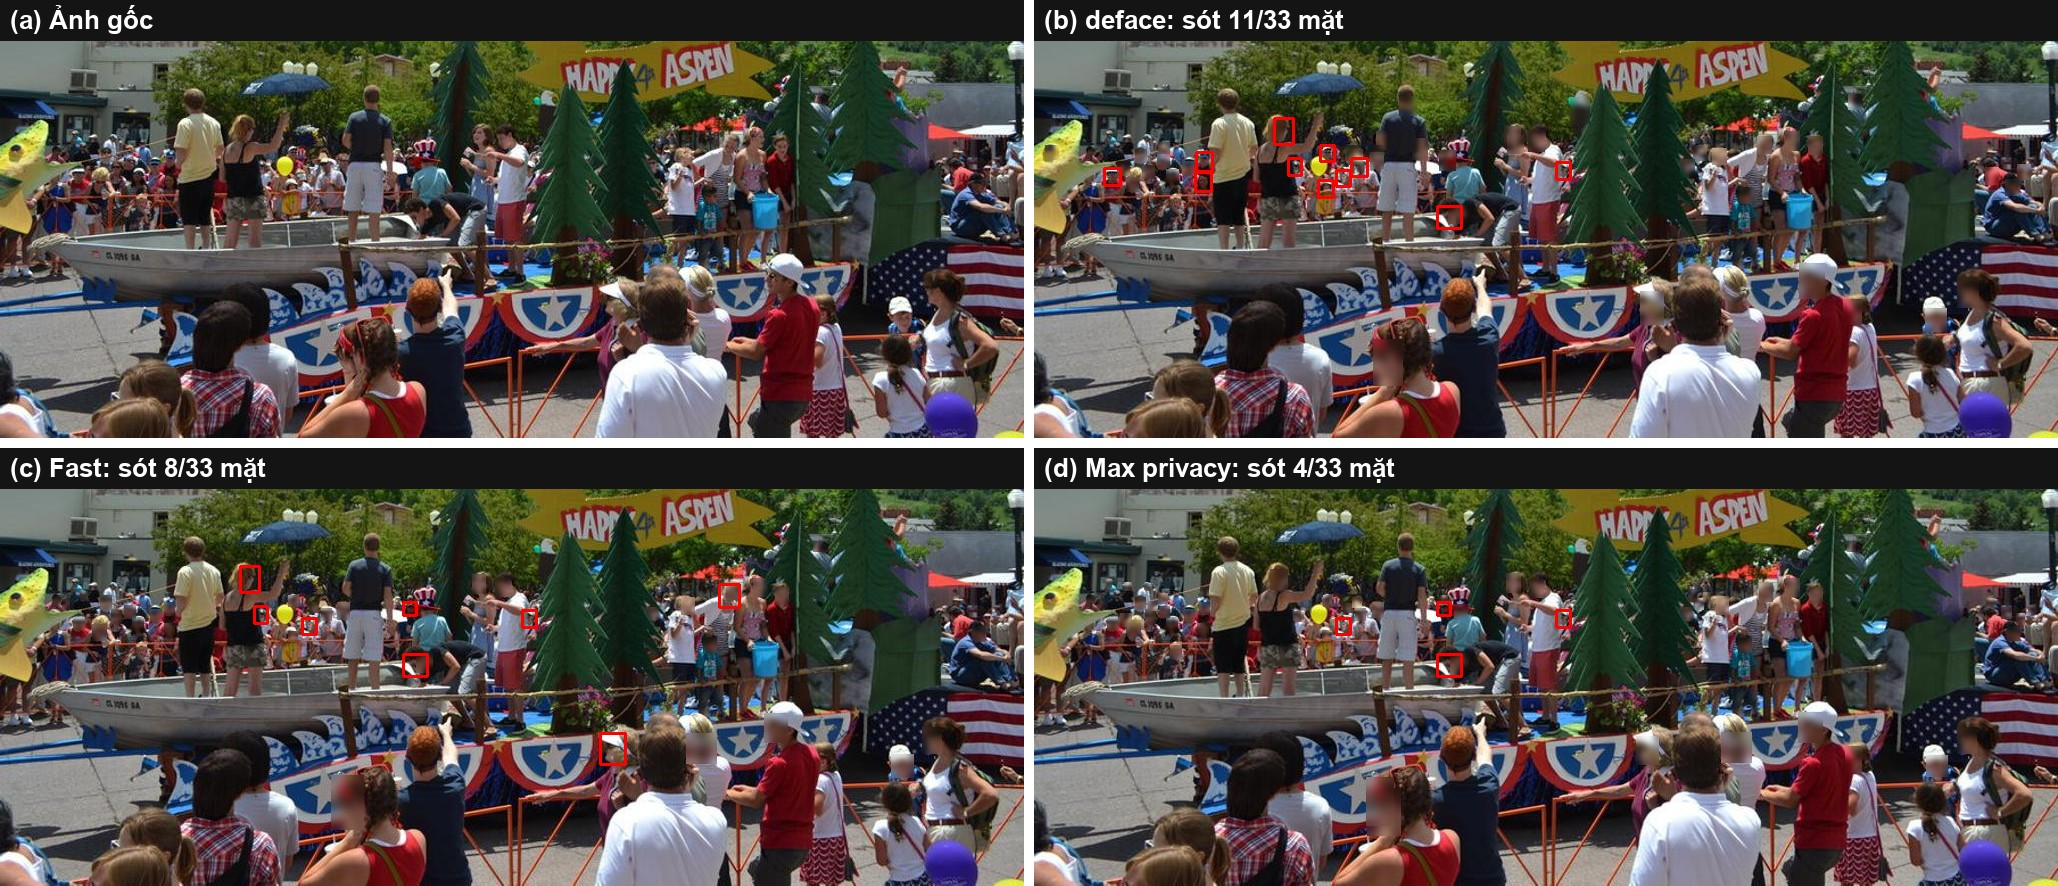
\includegraphics[width=0.98\textwidth]{figures/hinh-4-9-truc-quan.jpg}\\[4pt]
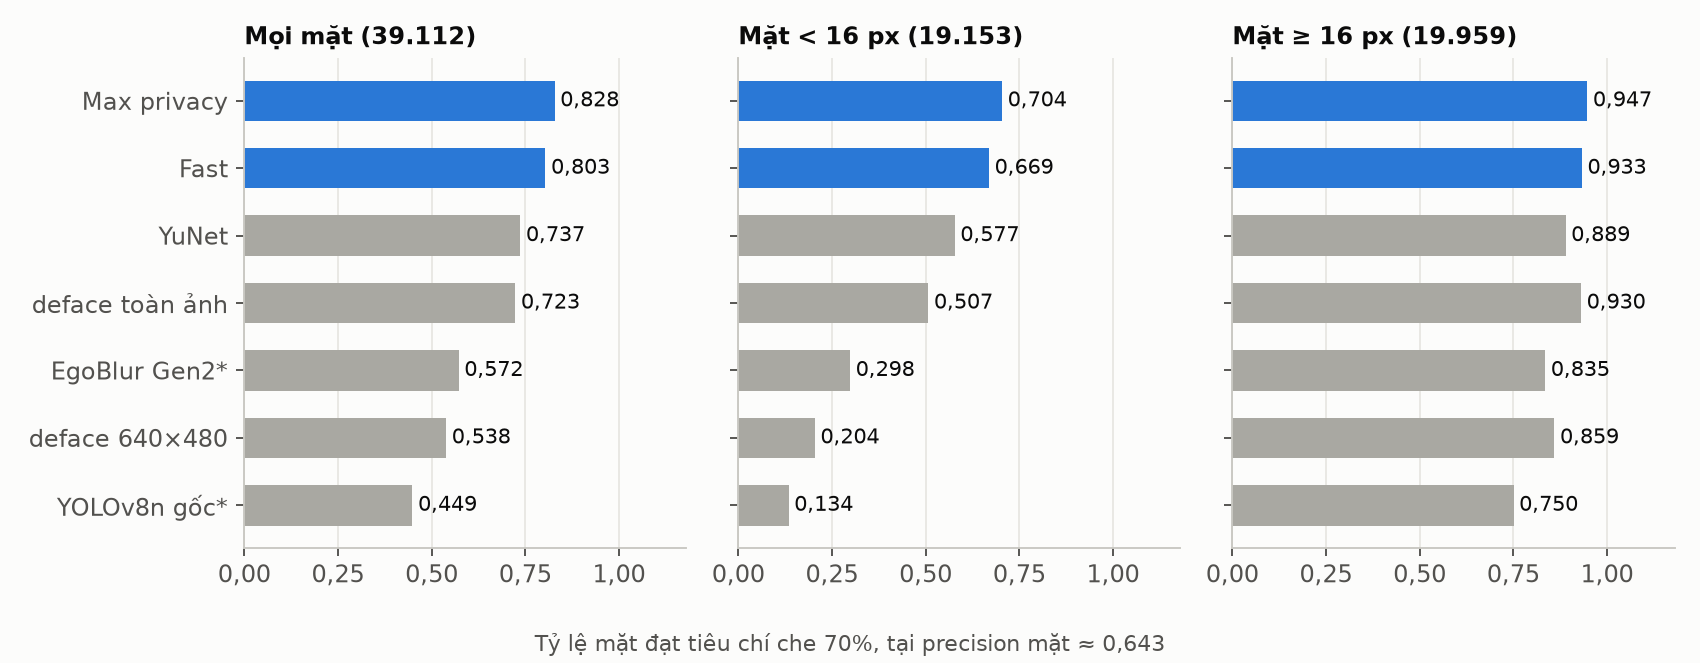
\includegraphics[width=0.85\textwidth]{figures/hinh-4-9-so-sanh-cong-cu.png}
\caption[So sánh RedactFunnel với các công cụ khác]{So sánh RedactFunnel với các công cụ khác. Trên: cùng một ảnh có 33 mặt được gán nhãn, khung đỏ là mặt chưa được che đủ 70\%. Dưới: tỷ lệ mặt đạt che ở precision 0,643. Dấu * là mô hình có precision cao hơn mức này}
\label{fig:4-9}
\end{figure}

\textbf{Khuôn mặt.} Ở đúng precision mặc định của deface (0,643), Max privacy che được 82,8\% số mặt và Fast 80,3\%, so với 72,3\% của deface. Khoảng cách chủ yếu nằm ở mặt dưới 16 px: 70,4\% và 66,9\% so với 50,7\%. Với mặt từ 16 px thì các công cụ gần nhau hơn: 94,7\%, 93,3\% và 93,0\%. Trong Hình~\ref{fig:4-9}, deface sót 11 mặt, Fast sót 8 và Max privacy sót 4. Ảnh này chỉ để minh hoạ: trên 60 ảnh đông người tương tự và ở ngưỡng mặc định của mỗi bên, deface và Fast gần bằng nhau (77,0\% và 77,3\%), còn Max privacy đạt 86,2\%.

\textbf{Biển số.} EgoBlur tìm được cả 500 biển cận cảnh, hơn cả hai chế độ của nhóm. Trên dashcam thì ngược lại: ở ngưỡng mặc định, EgoBlur bỏ sót 81,2\% biển trên clip dashcam 1, trong khi Engine với YOLO26s trước bước 8 chỉ bỏ sót 10,6\%. Hạ ngưỡng của EgoBlur xuống thấp nhất, bỏ sót còn 16,9\% nhưng chỉ che đầy đủ 30,8\% vì hộp không được nới.

\textbf{Trên cùng các clip.} Với clip điện thoại, deface khá gần Engine: trên clip 2a, tỷ lệ che đủ là 93,4\% so với 93,3\% của nhóm, nhưng deface còn bỏ sót 1,5\% mặt so với 0\%. Ở clip 1 và 2b, Engine đạt 92,1\% và 94,6\%, deface đạt 90,5\% và 85,1\%. Với mặt trong hai clip dashcam, Engine đạt 100\%, deface 80,9\% và 98,8\%, EgoBlur 51,1\% và 95,5\%. Các phép đo này dùng mô hình trước bước 8.

\textbf{Tốc độ.} deface xử lý 614 ảnh/phút trên GPU ở toàn ảnh và 294 ảnh/phút trên CPU khi chạy trực tiếp trên tệp cục bộ. Engine được đo qua cả hệ thống với ba worker: 1.646 ảnh/phút (Fast) và 1.232 ảnh/phút (Max privacy). Hai cách đo khác nhau nên không so trực tiếp. Nếu chia cho từng worker thì mỗi worker của nhóm (khoảng 550 và 410 ảnh/phút) chậm hơn một tiến trình deface.

\subsection{OCR biển số và whitelist biển số}

Để miễn che một biển số cần hai bước: đọc chuỗi và so chuỗi. Bản đầu tiên của Engine thử lần lượt PaddleOCR, EasyOCR và Tesseract, nhưng các thư viện này không được cài trong ảnh container nên luôn trả về rỗng và không biển nào được miễn che. Nhóm làm lại bước này từ đầu, so từng cách đọc trên 40 biển rồi kiểm tra trên 40 biển khác.

RapidOCR chạy đầy đủ chỉ đọc đúng 21/40 biển, EasyOCR 8/40. Vấn đề của RapidOCR nằm ở bước phát hiện chữ: nó tách một dòng thành nhiều mảnh chồng nhau nên ký tự bị lặp. Vì YOLO đã cắt sẵn biển, nhóm bỏ bước này và đọc nguyên vùng, kết quả lên 28/40 nhưng biển hai dòng thất bại. Đọc cả nguyên vùng lẫn hai nửa rồi chọn cách có điểm cao hơn đạt 37/40, kéo ngang thêm 1,3 lần thì đạt 40/40 ở cả hai nhóm biển (Hình~\ref{fig:4-10}).

\begin{figure}[!htp]
\centering
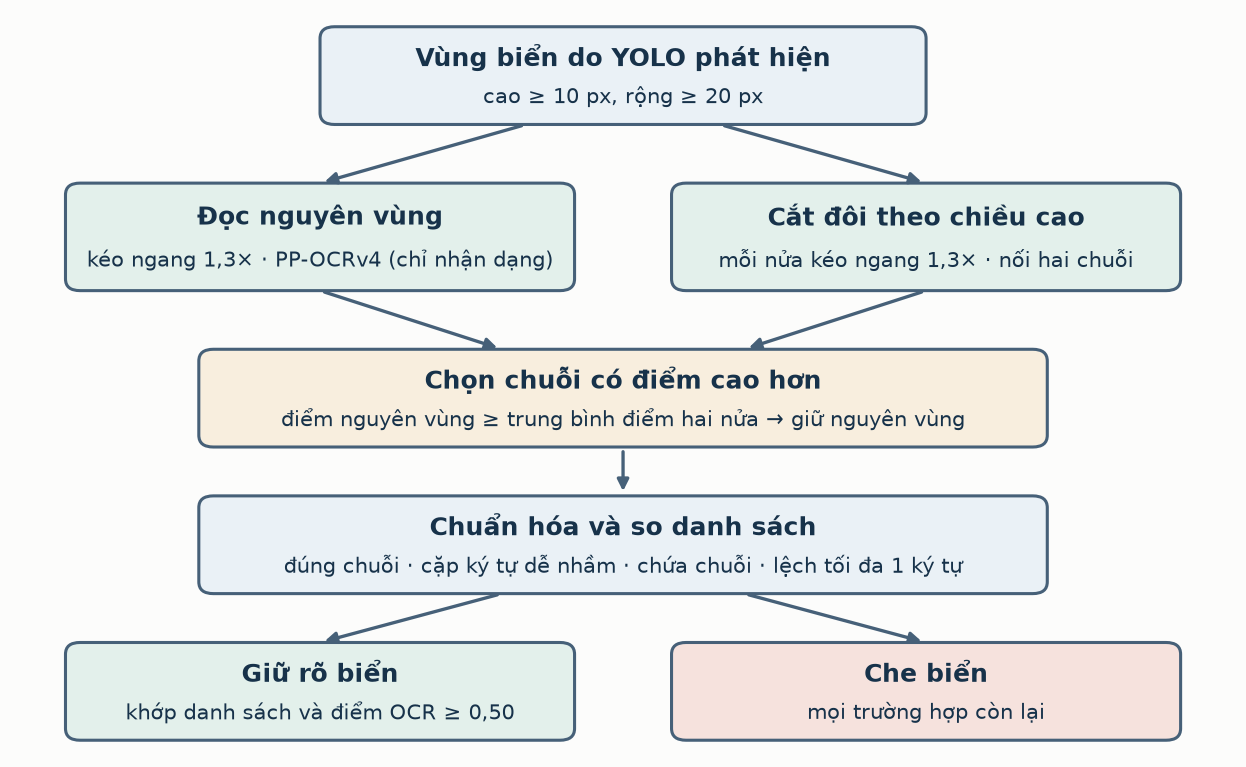
\includegraphics[width=0.8\textwidth]{figures/hinh-4-10-ocr-bien-so.png}
\caption[Quy trình đọc và so khớp biển số]{Quy trình đọc và so khớp biển số. Khi OCR lỗi hoặc không đọc được, biển mặc định bị che}
\label{fig:4-10}
\end{figure}

\begin{table}[!htp]
\centering\bangnho
\caption{So sánh các phương pháp OCR biển số}\label{tab:4-6}
\begin{tabular}{|L{4.3cm}|C{1.7cm}|C{2.0cm}|C{1.7cm}|C{2.6cm}|C{1.8cm}|}
\hline
\dongdau \textbf{Phương pháp} & \textbf{UET (80)} & \textbf{trungdinh (536)} & \textbf{2 dòng (440)} & \textbf{Thời gian / biển} & \textbf{RAM tăng thêm} \\ \hline
Tesseract & 35,0\% & 17,0\% & 12,7\% & 75 ms & 40 MB \\ \hline
RapidOCR đầy đủ & 53,8\% & 65,9\% & 79,1\% & 1.490--2.364 ms & 537 MB \\ \hline
Chỉ nhận dạng, nguyên vùng & 75,0\% & 17,5\% & 0,0\% & 45 ms & 63 MB \\ \hline
Chỉ nhận dạng, nguyên vùng hoặc chia đôi & 92,5\% & 88,1\% & 85,9\% & 120 ms & 67 MB \\ \hline
\textbf{Như trên, kéo ngang 1,3 lần (Engine)} & \textbf{100\%} & \textbf{88,6\%} & \textbf{86,6\%} & 120 ms & 66 MB \\ \hline
\end{tabular}
\end{table}

Mọi dòng trong Bảng~\ref{tab:4-6} được đo trên cùng một máy Core Ultra 5 125H giới hạn 4 luồng, chỉ dùng CPU. Tesseract đọc kém nhất trên tập UET và gần như không đọc được biển hai dòng. RapidOCR đầy đủ khá hơn nhưng chậm hơn cách của nhóm hơn 10 lần và tốn thêm khoảng 470 MB RAM. Gộp cả hai tập, Engine đọc đúng 555/616 biển (90,1\%).

Trong 61 biển đọc sai, 59 biển có hai dòng và 50 biển chỉ sai đúng một ký tự. Khoảng một phần tư số lỗi đến từ nhãn của tập dữ liệu bị thiếu ký tự. Các cặp dễ nhầm nhất là 2 với Z và 1 với 7. Tập UET chỉ có 16 biển hai dòng nên con số 100\% không có nghĩa là biển xe máy luôn đọc được.

\textbf{Quy tắc so khớp.} Vì OCR hay sai một ký tự, so chuỗi tuyệt đối sẽ che nhầm biển của chính chủ xe. Biển được miễn che khi điểm OCR từ 0,50 và thoả một trong các điều kiện: trùng chuỗi; trùng sau khi quy đổi các ký tự dễ nhầm (O và D thành 0, G thành 6, B thành 8, I thành 1, S thành 5, Z thành 2); biển trong danh sách nằm trọn trong chuỗi đọc được; hoặc cùng hai số đầu và chỉ khác tối đa một ký tự. Nhóm kiểm tra các quy tắc trên 616 biển, lần lượt coi mỗi biển là chủ xe và các biển còn lại là người lạ:

\begin{center}
\bangfont
\begin{tabular}{|L{5.0cm}|C{3.0cm}|C{3.2cm}|C{3.3cm}|}
\hline
\dongdau \textbf{Bộ so khớp} & \textbf{Giữ đúng biển chủ xe} & \textbf{Biển bị một biển khác khớp} & \textbf{Người lạ lọt, danh sách 20 biển} \\ \hline
Chỉ trùng chuỗi & 90,1\% & 0,32\% & 0,012\% \\ \hline
Bản cũ, cho sai 2--3 ký tự & 97,7\% & 46,1\% & 3,0\% \\ \hline
Cho sai tối đa 2 ký tự & 97,7\% & 7,1\% & 0,30\% \\ \hline
\textbf{Hiện tại, sai tối đa 1 ký tự} & \textbf{97,4\%} & \textbf{0,97\%} & \textbf{0,036\%} \\ \hline
\end{tabular}
\end{center}

Bản cũ cho phép sai 2--3 ký tự khiến gần một nửa số biển khớp với một biển khác. Siết xuống một ký tự chỉ mất 0,3 điểm phần trăm của chủ xe nhưng giảm tỷ lệ người lạ lọt khoảng 80 lần. Phần lọt còn lại là những cặp biển chỉ khác nhau một ký tự, không quy tắc mờ nào phân biệt được. Các biển trong tập này đều là ảnh cận cảnh, kết quả với biển nhỏ trên đường được xem ở mục 4.8.

\subsection{Whitelist khuôn mặt}

Nhóm đánh giá trên LFW với 600 chủ thể. Ảnh kiểm tra của mỗi người được so với một hoặc ba ảnh mẫu, lấy điểm cosine cao nhất. TAR là tỷ lệ ảnh của chủ thể đạt ngưỡng, tính trên 600 ảnh. FAR là tỷ lệ phép so với người khác đạt ngưỡng, tính trên 1.797.600 phép so. Kết quả ở ngưỡng 0,45 như Bảng~\ref{tab:4-7}.

\begin{table}[!htp]
\centering\bangfont
\caption[Độ chính xác whitelist khuôn mặt theo phương pháp căn chỉnh]{Độ chính xác whitelist khuôn mặt theo phương pháp căn chỉnh (ngưỡng 0,45)}\label{tab:4-7}
\begin{tabular}{|L{4.4cm}|C{1.4cm}|C{1.4cm}|C{3.3cm}|L{3.9cm}|}
\hline
\dongdau \textbf{Phương pháp} & \textbf{Ảnh mẫu} & \textbf{TAR} & \textbf{FAR (số phép so)} & \textbf{Ghi chú} \\ \hline
Hộp YOLO, không căn chỉnh & 1 & 38,8\% & $4{,}7\times10^{-5}$ (84) & Bản đầu tiên \\ \cline{2-5}
 & 3 & 64,5\% & $1{,}6\times10^{-4}$ (290) & \\ \hline
Hộp nới 15\% & 1 & 59,5\% & $1{,}5\times10^{-4}$ (273) & \\ \hline
Hộp nới 30\% & 1 & 67,8\% & $2{,}0\times10^{-3}$ (3.614) & FAR tăng khoảng 43 lần \\ \hline
Hộp nới 15\%, tô phẳng nền & 1 & 57,3\% & $4{,}8\times10^{-4}$ (865) & Nền không phải nguyên nhân \\ \hline
YuNet trên cả ảnh & 1 & 87,0\% & $3{,}9\times10^{-6}$ (7) & Mức tham khảo cao nhất \\ \cline{2-5}
 & 3 & 96,5\% & $3{,}9\times10^{-6}$ (7) & \\ \hline
\textbf{Engine, Max privacy} & 1 & \textbf{84,3\%} & $3{,}3\times10^{-6}$ (6) & YuNet trên vùng mặt \\ \cline{2-5}
 & 3 & \textbf{96,2\%} & $3{,}3\times10^{-6}$ (6) & \\ \hline
Engine, Fast & 1 & 83,5\% & $3{,}3\times10^{-6}$ (6) & \\ \cline{2-5}
 & 3 & 95,7\% & $3{,}3\times10^{-6}$ (6) & \\ \hline
\end{tabular}
\end{table}

Căn chỉnh bằng YuNet là thay đổi có tác dụng lớn nhất: với một ảnh mẫu, TAR tăng từ 38,8\% lên 84,3\% trong khi số phép so nhầm giảm từ 84 xuống 6. Nới hộp cũng tăng TAR nhưng kéo FAR tăng theo, nên bị loại. Đổi bộ phát hiện gần như không ảnh hưởng: sáu mô hình lệch nhau nhiều nhất 2 điểm phần trăm. Hình~\ref{fig:4-11} cho thấy hai phân bố tách nhau khá rõ quanh ngưỡng 0,45, và các mặt nằm trong vùng $\pm0{,}05$ được đưa vào mục cần xem lại.

\begin{figure}[!htp]
\centering
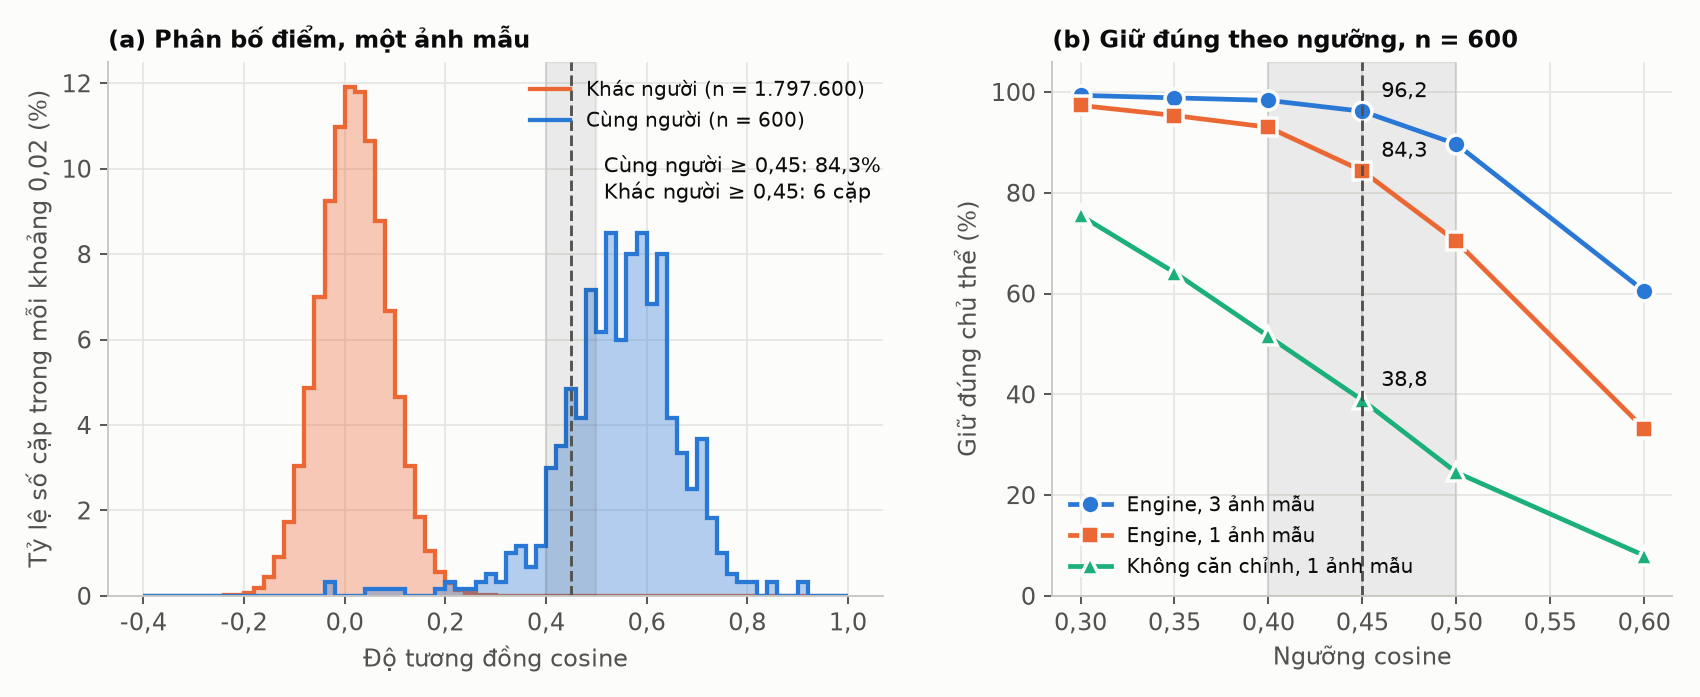
\includegraphics[width=0.98\textwidth]{figures/hinh-4-11-nguong-cosine.png}
\caption[Phân bố cosine similarity của cặp cùng người và khác người]{(a) Phân bố cosine similarity của cặp cùng người và khác người, một ảnh mẫu. (b) Tỷ lệ giữ đúng chủ thể theo ngưỡng. Vạch đứt là ngưỡng 0,45, vùng xám là vùng cần xem lại}
\label{fig:4-11}
\end{figure}

\textbf{Kích thước khuôn mặt.} Mặt càng nhỏ càng khó giữ đúng chủ thể. Với một ảnh mẫu, TAR giảm từ 84,3\% xuống 64,0\% ở 64 px, 34,7\% ở 40 px và 6,0\% ở 24 px. Dùng ba ảnh mẫu thì các mức là 96,2\%, 86,5\%, 59,3\% và 17,0\%. Nếu chấp nhận mức người lạ 1/10.000, ngưỡng ở 40 px có thể hạ xuống 0,327 và TAR tăng lên 72,7\% (Hình~\ref{fig:4-12}). Nhóm chưa áp dụng ngưỡng theo kích thước vì LFW chỉ có mặt chính diện, chưa đủ cơ sở cho góc nghiêng và khuôn mặt người Việt.

\begin{figure}[!htp]
\centering
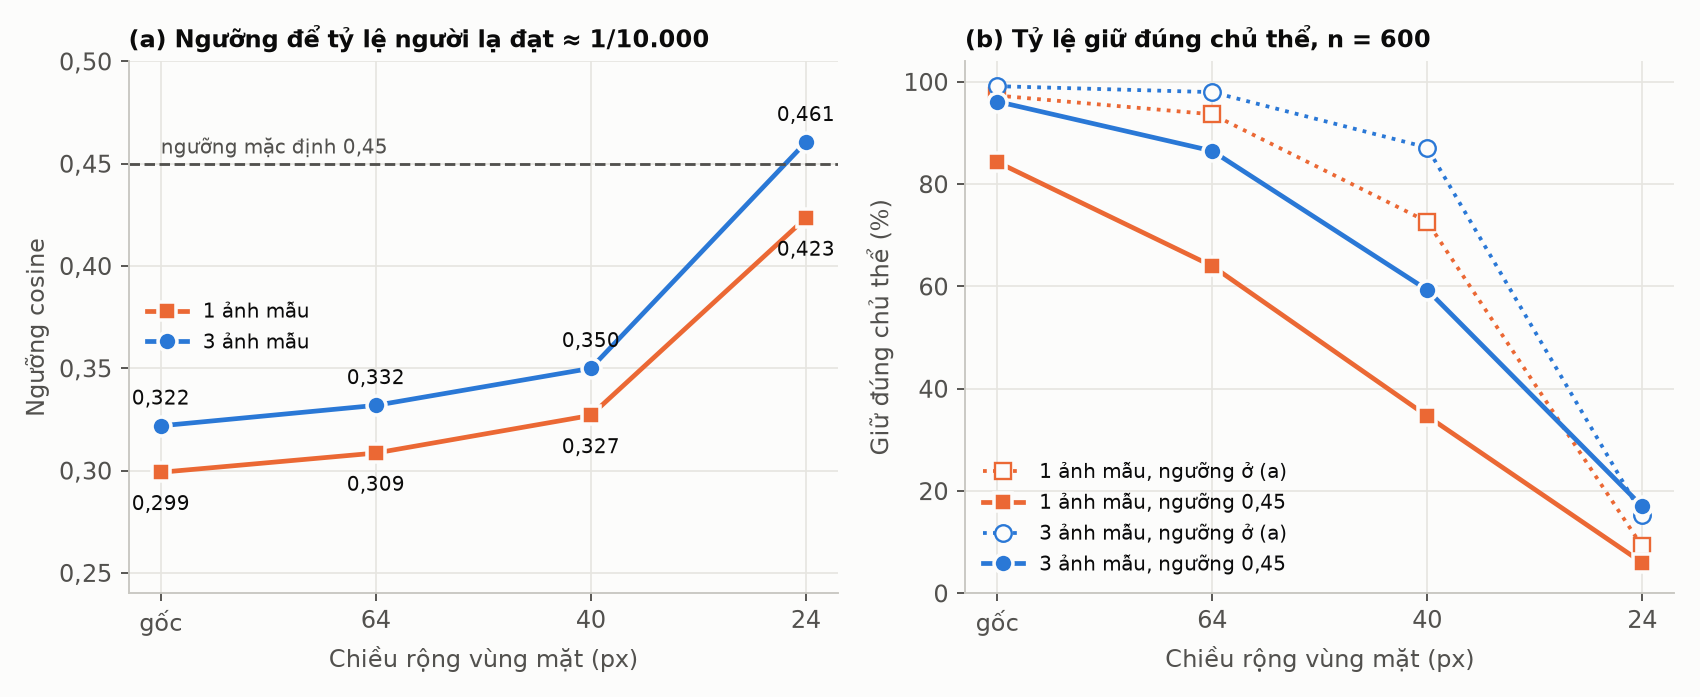
\includegraphics[width=0.98\textwidth]{figures/hinh-4-12-nguong-theo-kich-thuoc.png}
\caption[Ngưỡng similarity theo kích thước khuôn mặt]{Ngưỡng similarity theo kích thước khuôn mặt. (a) Ngưỡng để tỷ lệ người lạ khoảng 1/10.000. (b) TAR tương ứng, so với ngưỡng cố định 0,45}
\label{fig:4-12}
\end{figure}

\textbf{Rủi ro nhận nhầm người lạ.} Với FAR khoảng 3 phần triệu, một video có 1.000 mặt lạ và danh sách 5 người có khoảng 1,7\% khả năng lọt ít nhất một người, nếu coi các phép so là độc lập. Khi lọt, cả đoạn quỹ đạo sẽ không được che, nên nhóm giữ ngưỡng 0,45 thay vì hạ xuống. Nhóm xem lại sáu cặp bị nhận nhầm trên LFW. Bốn cặp đến từ một ảnh có hai người đứng cạnh nhau, hệ thống lấy nhầm mặt của người còn lại. Một cặp dùng ảnh mà danh sách đính chính của LFW ghi là gán sai tên. Chỉ còn một cặp chưa rõ nguyên nhân, nên tỷ lệ nhận nhầm thực tế có thể còn thấp hơn. Trường hợp này cũng cho thấy ảnh mẫu nên chỉ có một khuôn mặt.

\subsection{Đánh giá trên video thực tế}

Đánh giá trên video kiểm tra toàn bộ Engine chứ không chỉ mô hình. Engine chạy trước trên từng clip, kết quả được đưa vào CVAT dưới dạng quỹ đạo để sửa tay và gán danh tính chủ thể hoặc người lạ. Với mỗi hộp nhãn ở mỗi khung, nhóm tính phần diện tích thực sự được che, gồm cả vết nội suy và vết giữ 200 ms. Tỷ lệ bỏ sót là tỷ lệ nhãn không được che chút nào, còn tỷ lệ giữ đúng là số khung của chủ thể được giữ rõ. Bảng~\ref{tab:4-8} so năm thời điểm: trước hai bản sửa Engine, sau hai bản sửa, sau khi sửa danh sách miễn che, và hai mô hình dashcam cuối cùng.

\begin{table}[!htp]
\centering\bangnho
\caption{Kết quả che và whitelist trên clip video (\%)}\label{tab:4-8}
\begin{tabular}{|L{2.1cm}|L{4.7cm}|C{1.3cm}|C{1.4cm}|C{1.5cm}|C{1.5cm}|C{1.2cm}|}
\hline
\dongdau \textbf{Clip} & \textbf{Chỉ số (số nhãn)} & \textbf{Trước sửa} & \textbf{Sau 2 bản sửa} & \textbf{Sửa miễn che} & \textbf{Max privacy} & \textbf{Fast} \\ \hline
Dashcam 1 & Biển bỏ sót (1.668) & 22,8 & 10,6 & 10,6 & \textbf{2,3} & 5,7 \\ \cline{2-7}
 & \quad rộng từ 40 px (1.627) & 21,8 & 9,8 & 9,8 & \textbf{2,3} & 5,3 \\ \cline{2-7}
 & \quad bị che một phần (219) & 55,7 & 30,6 & 30,6 & \textbf{11,9} & 21,5 \\ \cline{2-7}
 & Biển che đủ 90\% (1.668) & 56,9 & 70,4 & 70,4 & 76,6 & 74,6 \\ \cline{2-7}
 & Mặt bỏ sót (481) & 0,0 & 0,0 & 0,0 & 0,0 & 8,9 \\ \cline{2-7}
 & Giữ đúng biển chủ xe (894) & 86,0 & 69,5 & 67,8 & 69,7 & 68,9 \\ \hline
Dashcam 2 & Biển bỏ sót, từ 40 px (64) & 73,4 & 32,8 & 32,8 & \textbf{9,4} & 9,4 \\ \cline{2-7}
 & Mặt bỏ sót (420) & 0,0 & 0,0 & 0,0 & 0,0 & 0,2 \\ \cline{2-7}
 & Giữ đúng biển chủ xe (1.245) & 87,9 & 75,0 & 75,0 & \textbf{89,2} & 83,8 \\ \hline
Điện thoại 1 & Mặt bỏ sót (828) & 1,9 & 0,0 & 0,0 & 0,0 & 0,7 \\ \cline{2-7}
 & Mặt che đủ 70\% & 90,1 & 92,1 & 92,1 & 91,4 & 90,2 \\ \cline{2-7}
 & Giữ đúng chủ thể (347) & 74,4 & 70,3 & 70,3 & 70,3 & 69,5 \\ \hline
Điện thoại 2a & Mặt bỏ sót (1.494) & 5,0 & 0,0 & 0,0 & 0,0 & 0,0 \\ \cline{2-7}
 & Mặt che đủ 70\% & 80,8 & 93,3 & 93,3 & 93,2 & 93,4 \\ \cline{2-7}
 & Giữ đúng chủ thể (549) & 71,2 & 60,1 & 59,4 & 58,3 & 61,6 \\ \hline
Điện thoại 2b & Mặt bỏ sót (1.074) & 4,8 & 0,4 & 0,4 & 0,4 & 2,1 \\ \cline{2-7}
 & Mặt che đủ 70\% & 85,5 & 94,6 & 94,6 & 92,9 & 90,6 \\ \cline{2-7}
 & Giữ đúng chủ thể (699) & 75,5 & 71,2 & 70,2 & 71,1 & 73,0 \\ \hline
Cả 5 clip & Khung người lạ bị giữ như chủ thể (6.031) & 2 & 5 & 5 & 15 & 11 \\ \hline
\end{tabular}
\end{table}

\textbf{Hai bản sửa Engine.} Khi chấm các clip này, nhóm phát hiện hai lỗi của luồng video: bộ lọc theo vị trí bỏ qua mặt người thật, và các phát hiện chưa được ByteTrack xác nhận bị loại trước bước che. Sau khi sửa, mặt bỏ sót ở clip điện thoại giảm từ 1,9--5,0\% xuống 0--0,4\%, biển bỏ sót ở clip dashcam 1 giảm từ 22,8\% xuống 10,6\%. Số đoạn bị lộ từ 200 ms trở lên ở clip này giảm từ 19 xuống 15. Đổi lại, tỷ lệ giữ đúng chủ thể giảm, vì các phát hiện mới tạo thành những đoạn rất ngắn, khó khớp danh sách miễn che nên bị che. Cách sửa được trình bày ở mục 5.3.

\textbf{Biển nhỏ và biển bị che.} Mô hình học từ ảnh cận cảnh nên trước bước 8 còn bỏ sót 9,8\% biển rộng từ 40 px trên clip dashcam 1. Sau khi học thêm khung dashcam, Max privacy chỉ còn 2,3\%, biển bị che một phần giảm từ 30,6\% xuống 11,9\%. Fast giảm từ 11,4\% xuống 5,3\%. Ở clip dashcam 2, Max privacy giảm từ 32,8\% xuống 9,4\%, nhưng clip này chỉ có 64 biển nên mỗi biển ứng với khoảng 1,5 điểm phần trăm. Mặt trái của bước 8 là mô hình nhận logo trắng trên đồng hồ xe của người quay thành biển (1.730 hộp với Max privacy và 269 hộp với Fast), gây che thừa nhưng không lộ thông tin.

\textbf{Giữ đúng chủ thể.} Tính chung, Max privacy giữ đúng 81,1\% khung biển của chủ xe và 66,5\% khung mặt của chủ thể, Fast là 77,6\% và 68,3\%. Việc chuyển sang đọc các vùng cắt rộng nhất giúp hai cấu hình trên clip dashcam 2 tăng từ 34\% lên 82\% và từ 38\% lên 84\%. Số khung người lạ bị giữ nhầm tăng từ 5 lên 15 (Max privacy) và 11 (Fast) trên 6.031 khung, đều nằm ở hai clip dashcam và phần lớn là biển đã được che một phần. Không có khuôn mặt người lạ nào bị giữ nhầm trong ba clip điện thoại.

\textbf{Điểm yếu của Fast.} Trên clip dashcam 1, Fast bỏ sót 8,9\% khung mặt (43/481), còn Max privacy không bỏ sót. Nếu người dùng ưu tiên an toàn cho video hành trình thì nên chọn Max privacy.

\textbf{Lọc mục cần xem lại.} Một video thử dài 18 giây ban đầu có tới 88 mục cần xem lại, quá nhiều để người dùng kiểm tra hết. Trong 260 quỹ đạo của video, 215 quỹ đạo ngắn hơn 0,5 giây và chỉ lệch điểm ở vài khung. Chỉ giữ quỹ đạo từ 0,5 giây còn 34 mục, thêm điều kiện có đoạn điểm thấp hoặc mất dấu từ 0,25 giây thì còn 7 mục. Những mục bị lọc khỏi danh sách vẫn được che bình thường.

\begin{figure}[!htp]
\centering
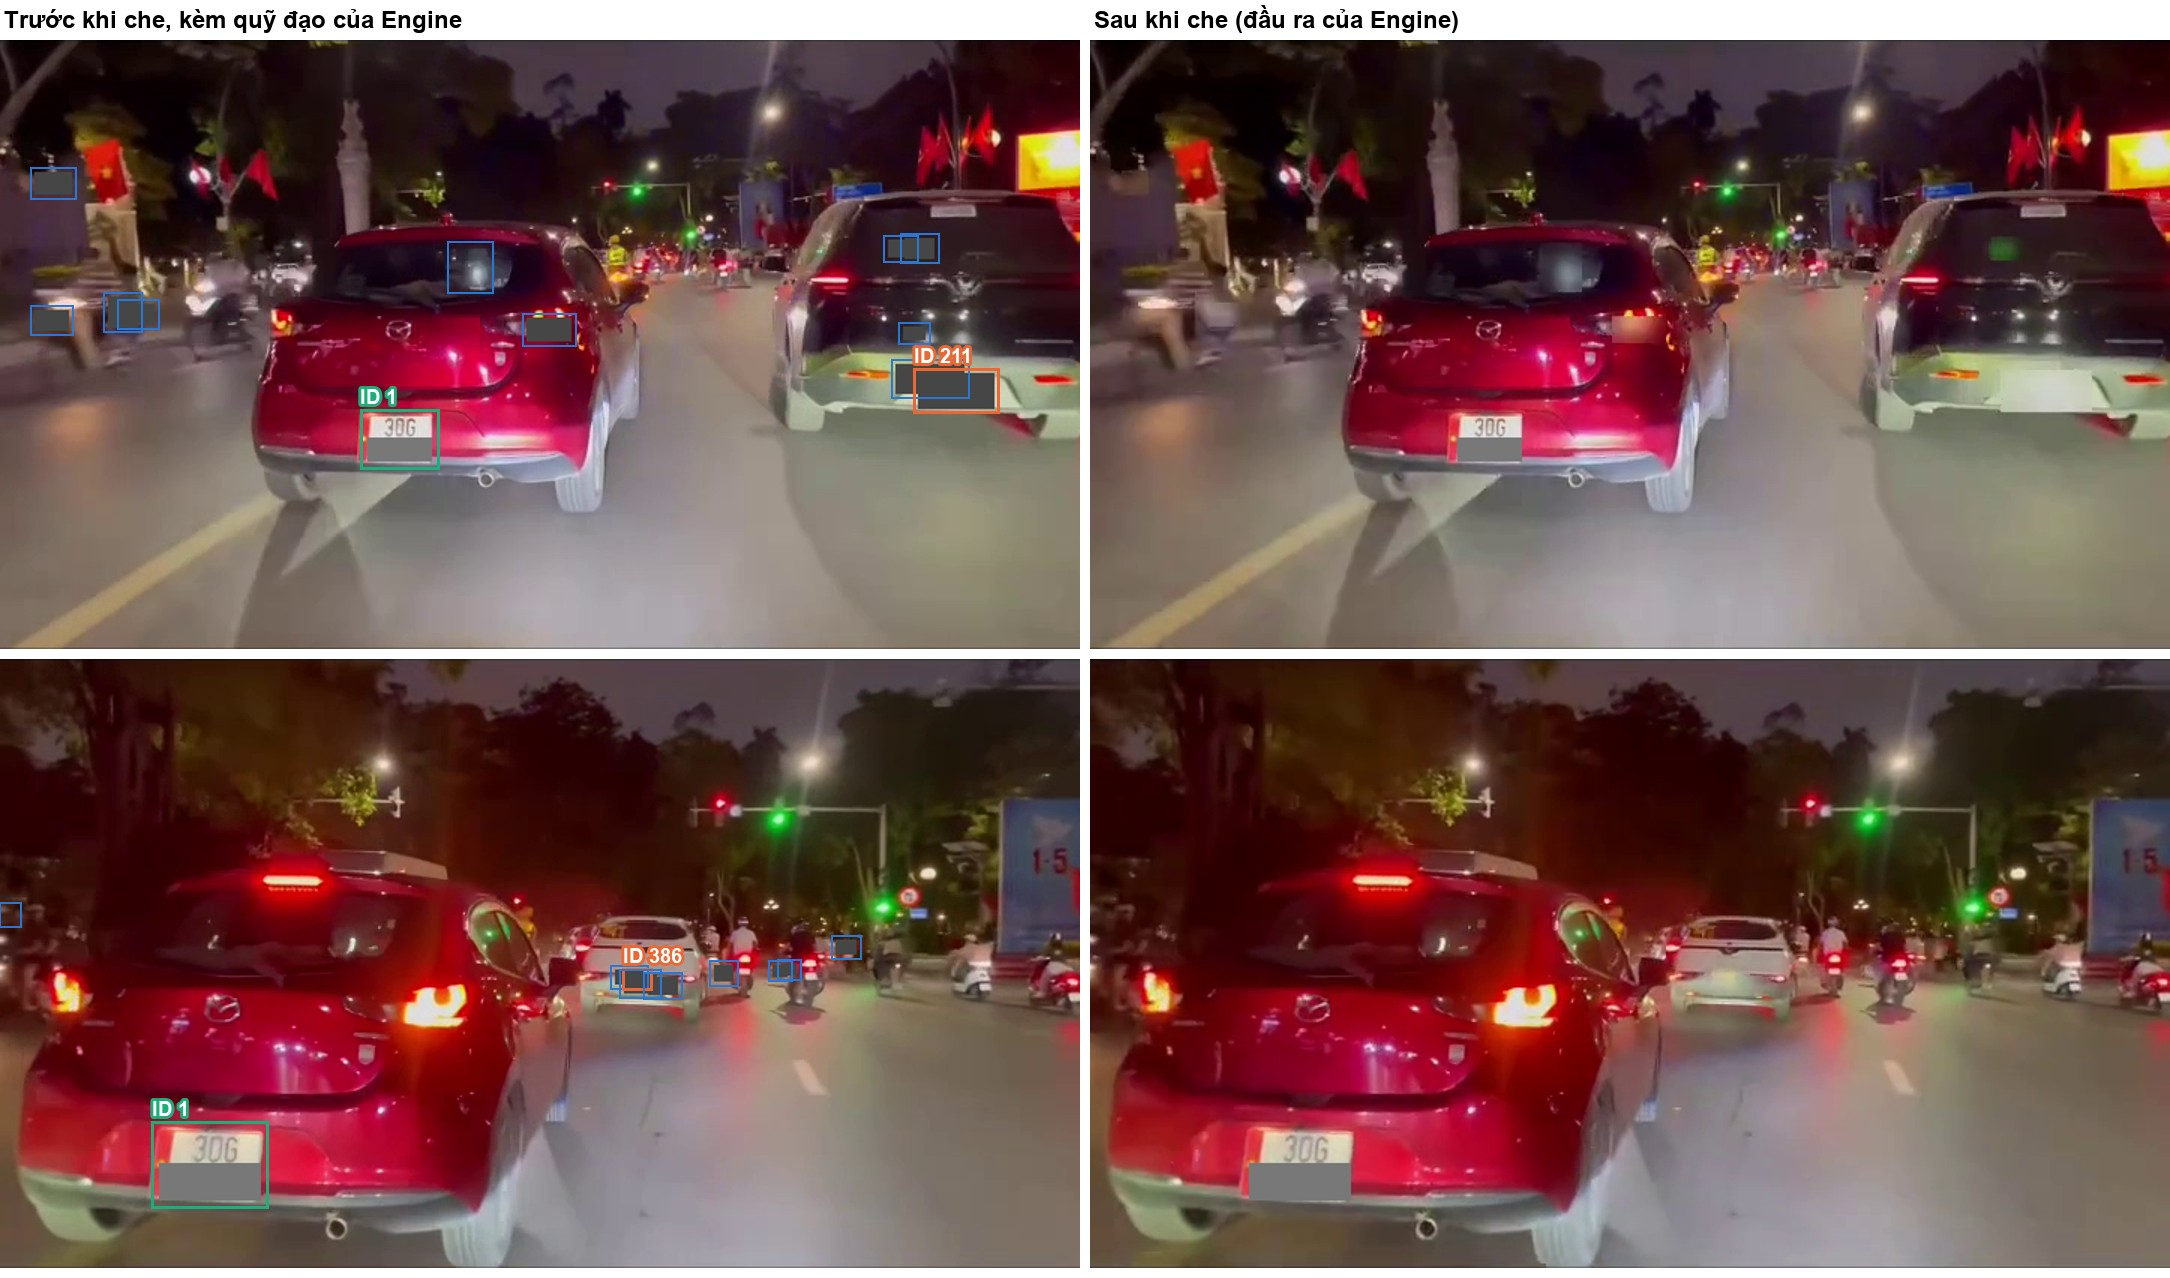
\includegraphics[width=0.98\textwidth]{figures/hinh-4-13-truoc-sau.jpg}
\caption[Ví dụ khung hình video trước và sau khi che]{Hai khung của clip dashcam 2, trước (trái) và sau khi che (phải), chế độ Max privacy. Khung xanh lá là quỹ đạo của chủ xe được giữ rõ, khung cam là phát hiện hiện tại, khung xanh dương là vết che giữ thêm 200 ms. Ô xám được thêm khi in để không lộ biển số}
\label{fig:4-13}
\end{figure}

Hình~\ref{fig:4-13} cho thấy biển của chủ xe được giữ rõ liên tục 234 khung, trong khi biển xe khác bị che. Nhiều vết che nhỏ là báo nhầm ánh đèn và phản chiếu, hệ quả của ngưỡng thấp ở chế độ Max privacy.

\textbf{Giới hạn.} Năm clip đều do nhóm chọn, mỗi clip chỉ một người gán nhãn và đã được dùng để sửa Engine. Một phần trường hợp che chưa đủ có thể do nhãn được CVAT nội suy giữa các khung chính. Vì vậy các tỷ lệ có thể thay đổi vài điểm khi có thêm dữ liệu.

\subsection{Chi phí suy luận trên CPU và GPU}

Bảng~\ref{tab:4-9} ghi thời gian và RAM của từng mô hình. Phần đầu đo trên cùng một máy để so được với nhau, phần sau là kết quả của cả Engine trên hai môi trường triển khai. Các nhóm dòng đo trên máy khác nhau nên không so chéo.

\begin{table}[!htp]
\centering\bangnho
\caption{Thời gian suy luận và RAM của từng mô hình trên CPU và GPU}\label{tab:4-9}
\begin{tabular}{|L{3.0cm}|C{1.7cm}|L{4.3cm}|C{2.7cm}|C{2.8cm}|}
\hline
\dongdau \textbf{Mô hình} & \textbf{Đầu vào} & \textbf{Runtime} & \textbf{Thời gian} & \textbf{RAM đỉnh} \\ \hline
\multicolumn{5}{|l|}{\textit{Từng mô hình, Core Ultra 5 125H giới hạn 4 luồng, chỉ CPU}} \\ \hline
YOLO26n & 960 & PyTorch, 2 luồng & 125 ms/ảnh & 602 MB \\ \hline
YOLO26n & 1280 & PyTorch, 2 luồng & 178 ms/ảnh & 672 MB \\ \hline
YOLO26s & 960 & PyTorch, 2 luồng & 240 ms/ảnh & 741 MB \\ \hline
YOLO26s & 1280 & PyTorch, 2 luồng & 389 ms/ảnh & 878 MB \\ \hline
ArcFace + YuNet & 112 & ONNX Runtime & 11,3 ms/mặt & 146 MB \\ \hline
RapidOCR & vùng biển & ONNX Runtime & 134 ms/biển & 260 MB \\ \hline
\multicolumn{5}{|l|}{\textit{Từng mô hình, máy laptop của nhóm}} \\ \hline
YOLO26n & 1280 & i5-12500H, PyTorch, 2 luồng & 153 ms/ảnh & --- \\ \hline
YOLO26s & 1280 & i5-12500H, PyTorch, 2 luồng & 387 ms/ảnh & --- \\ \hline
deface (CenterFace) & toàn ảnh & i5-12500H, ONNX, 2 luồng & 215 ms/ảnh & --- \\ \hline
YOLO26n & 1280 & RTX 3050, PyTorch & 20,4 ms/khung & --- \\ \hline
ArcFace + YuNet & 112 & ONNX Runtime CPU & 13,4 ms/mặt & --- \\ \hline
RapidOCR & vùng biển & ONNX Runtime CPU & 69,3 ms/biển & --- \\ \hline
\multicolumn{5}{|l|}{\textit{Cả Engine, không có danh sách miễn che}} \\ \hline
Fast & 1280 & RTX 3050, 3 worker & p50 61--65 ms & 1.274--1.337 MiB \\ \hline
Max privacy & 1280 & RTX 3050, 3 worker & p50 102--104 ms & 1.331--1.376 MiB \\ \hline
Fast & 1280 & i5-7200U, 2 worker & p50 0,96--1,20 s & 827--870 MiB \\ \hline
Max privacy & 1280 & i5-7200U, 2 worker & p50 2,85--2,99 s & 962--1.149 MiB \\ \hline
\end{tabular}
\end{table}

\textbf{Kích thước đầu vào và RAM.} Giảm từ 1280 xuống 960 px giúp YOLO26n nhanh hơn khoảng 30\% và YOLO26s nhanh hơn khoảng 38\%, nhưng như Bảng~\ref{tab:4-3}, tỷ lệ mặt được che giảm 6,7 điểm phần trăm, nên nhóm vẫn giữ 1280 px. Một tiến trình chỉ chạy YOLO cần 0,6--0,9 GB RAM, trong đó khoảng 0,33 GB là của Python và PyTorch. Đây là lý do worker chỉ giữ một mô hình YOLO trong bộ nhớ. Trọng số được đóng gói sẵn trong ảnh container nên pod không phải tải mô hình khi khởi động.

\textbf{CPU so với GPU.} Trên GPU, Max privacy chậm hơn Fast khoảng 1,7 lần. Trên máy lab chỉ có CPU, khoảng cách là 3 lần. Như vậy cái giá của chế độ an toàn hơn phụ thuộc nhiều vào phần cứng.

\textbf{Chi phí của danh sách miễn che.} Trên máy có GPU, chỉ YOLO chạy bằng GPU, còn YuNet, ArcFace và RapidOCR chạy trên CPU của worker. Khi thêm một ảnh mẫu khuôn mặt, tốc độ của Fast giảm từ 1.646 xuống 309 ảnh/phút, với danh sách hai biển còn 392 ảnh/phút. Max privacy giảm từ 1.232 xuống 262 và 309 ảnh/phút. Khi có danh sách khuôn mặt, RAM của worker ảnh lên 1.532 MiB, rất sát giới hạn 1.536 MiB.

\textbf{Video.} Nhóm chạy Fast trên đoạn 10 giây (300 khung) của clip dashcam 1 ở ba độ phân giải, YOLO chạy trên RTX 3050. Danh sách miễn che gồm một mặt và một biển không có trong clip, tức trường hợp tốn thời gian nhất:

\begin{center}
\bangfont
\begin{tabular}{|L{3.2cm}|C{2.4cm}|C{2.6cm}|C{3.0cm}|C{3.3cm}|}
\hline
\dongdau \textbf{Độ phân giải} & \textbf{Miễn che} & \textbf{Tốc độ} & \textbf{Thời gian xử lý} & \textbf{Trong đó OCR biển} \\ \hline
854$\times$480 & không & 36,6 fps & 8,2 s & --- \\ \cline{2-5}
 & có & 5,6 fps & 53,6 s & 44,1 s \\ \hline
1280$\times$720 & không & 27,6 fps & 10,9 s & --- \\ \cline{2-5}
 & có & 2,6 fps & 113,7 s & 101,1 s \\ \hline
1920$\times$1080 & không & 15,6 fps & 19,3 s & --- \\ \cline{2-5}
 & có & 2,2 fps & 139,6 s & 119,8 s \\ \hline
\end{tabular}
\end{center}

Ở 1080p, danh sách miễn che làm thời gian tăng từ 19,3 lên 139,6 giây, gần như toàn bộ do OCR biển số. Engine đọc tối đa sáu vùng cắt mỗi quỹ đạo và chỉ dừng sớm khi khớp, trong khi đoạn này có tới 711 quỹ đạo. RAM của tiến trình lên tới 1.968 MB, sát giới hạn 2.048 MiB của worker video, nên nhóm chưa thể khẳng định pod an toàn với video dài hơn.

\subsection{Kết luận chương}

\textbf{Về phát hiện và che.} Từ mô hình có sẵn đến YOLO26s tinh chỉnh ở 1280 px, tỷ lệ mặt đạt tiêu chí che tăng từ 44,9\% lên 79,5\% ở cùng mức precision khoảng 0,78, và lên 83,4\% khi dùng ngưỡng của Max privacy. Kích thước đầu vào ảnh hưởng nhiều hơn cỡ mô hình. Trên video, hai bản sửa Engine đưa mặt bỏ sót trên clip điện thoại xuống 0--0,4\%, còn khung dashcam giảm biển bỏ sót từ 9,8\% xuống 2,3\% (Max privacy) và từ 11,4\% xuống 5,3\% (Fast) với biển rộng từ 40 px.

\textbf{Về danh sách miễn che.} Với khuôn mặt, hệ thống giữ đúng chủ thể 84,3\% khi có một ảnh mẫu và 96,2\% khi có ba ảnh, nhưng giảm mạnh với mặt nhỏ và chỉ đạt 58--73\% trên video điện thoại. Với biển số, bộ so khớp giữ đúng 97,4\% biển cận cảnh và 69--89\% khung biển trong video. Phần lớn sai sót là che nhầm chủ thể, tức sai về phía an toàn.

\textbf{So với mục tiêu ở Chương 1.} Mục tiêu mAP\textsubscript{50} từ 85\% đạt ở trung bình hai lớp (87,0\% và 86,5\%), nhưng riêng lớp mặt mới đạt 77,3\% và 74,8\%. Mục tiêu giữ đúng người quen 85\% đạt khi có ba ảnh mẫu, gần đạt với một ảnh mẫu và chưa đạt trên video.

\textbf{Các điểm còn yếu.} Mặt dưới 16 px mới được che 71,4\% ở Max privacy, vì ở kích thước này gần như không còn chi tiết để nhận ra. Biển bị che một phần vẫn bị bỏ sót 11,9\% do dữ liệu huấn luyện hầu như không có mẫu như vậy. Chế độ Fast còn bỏ sót 8,9\% khung mặt trên một clip dashcam, và có 11--15 khung người lạ bị giữ như chủ thể. Ngoài ra, bộ đánh giá ảnh và các clip đều đã được dùng khi chọn mô hình, nên kết quả cần được kiểm chứng thêm trên dữ liệu mới.
